% !TEX root =  manuscript_arxiv.tex
\section{Introduction}
\section{Introduction}
\label{sec:introduction}
Hierarchical Reinforcement Learning (HRL) seeks to address the scalability problem of Reinforcement Learning (RL) by introducing layers of abstraction over the decision process, enabling  general sweeping decisions over large epochs and smaller specific decisions on finer (more granular) epochs \citep{SUTTON1999181, Barto2003}. The success of HRL relies on discovering suitable abstractions. 
In the literature, the problem of discovering suitable abstractions has been tackled both separately and in conjunction (in a single end-to-end process) with learning the optimal policy \citep{Barto2003}.
In specific instances where expert demonstrations are available, the process of discovering abstractions and learning optimal policies can be accelerated via \emph{Hierarchical Imitation Learning} (HIL).
Specifically, HIL involves computing a hierarchy of policies from expert demonstrations and is the extension of \emph{Imitation Learning} (IL) to HRL.
In this paper, we develop a novel HIL approach for the HRL with options framework of \citep{SUTTON1999181}.

The HRL with options framework proposed by \cite{SUTTON1999181} involves a two-tiered hierarchy of policies, with a high-level policy governing ``options'' or decision as to which of a finite set of low-level policies are used to select actions.
A key challenge of HIL in this options framework is that in practice, only (low-level) states and actions are directly observed through expert demonstrations, not the (high-level) options.
The options thus constitute hidden (or latent) variables, and so recent HIL works have drawn inspiration from Expectation-Maximization (EM) techniques for learning Hidden Markov models (HMMs) and other latent variable models \citep{Daniel2016,zhiyu20,Giammarino_2021}.
These EM techniques process state-action pairs from expert demonstrations with a Bayesian smoother to compute a surrogate function for the (log)likelihood, and subsequent maximization of this surrogate function over the policy space.
Whilst local-convergence theoretical guarantees have recently been shown for such an EM approach in the context of HIL~\citep{zhiyu20}, the nature of EM techniques as local-search procedures means that they are prone to convergence to local (non-global) maxima, and slow convergence with associated high computational expense.

In HMMs and other specific classes of latent variable models, \emph{methods of moments} have been developed to overcome convergence issues inherent with EM techniques \citep{hsu08,HsuKakade13,Mattila2020,Mattila2015,Mattila2017,Anandkumar2014,Parikh2012}.
These moment methods are free of local convergence problems \citep{Mattila2020,Anandkumar2014}, and often offer much faster practical convergence with less computational expense \citep{Mattila2015,Mattila2017}.
Moment methods have therefore been used both by themselves and as initialization algorithms for EM techniques (cf.~\citep{Zhang2016}).
Nevertheless, moment methods have not previously been investigated for HIL in the options framework.
%These methods of moments process a single sweep through the dataset and compile various statistics (moments) that can be used to compute the parameters of the model. 
%An few examples of moments are the second or third order consecutive moments, where the joint probability of pairs or triplets of consecutive observations are examined \cite{hsu08}. 
%Unlike EM methods, 

The key contribution of this paper is the development of a new method of moments for HIL in the HRL options framework of \citep{SUTTON1999181}. Inspired by the method of moments for HMMs developed in \citep{hsu08}, our method of moments for HIL offers global convergence under mild regularity and non-degeneracy conditions, and has the practical advantage of only requiring a single pass through the expert demonstrations.
It therefore serves as both a useful alternative and complementary technique to the previously developed but locally-convergent EM algorithms of \citep{Daniel2016,Giammarino_2021, zhiyu20}.

\emph{Notation:}
Uppercase letters denote random variables, lowercase letters denote realizations. Uppercase bold letters denote matrices, lowercase bold letters denote vectors. Superscript on a quantity acts like a label in case there are many quantities with the same symbol. Subscript on a quantity denotes it being a subclass of the original quantity.
The Kronecker product $\otimes$ is defined as
\[
    \bm{A}\otimes \bm{B}=\bmat{a_{11}\bm{B}&\dots&a_{1n}\bm{B}\\ \vdots&\ddots&\vdots\\ a_{m1}\bm{B}&\dots&a_{mn}\bm{B}},
\]
where $\bm A$ is a $m\times n$ matrix, $\bm B$ is a $p\times q$ matrix, 
and $\bm{A}\otimes \bm{B}$ is a $mp\times nq$ matrix.
The Hadamard (element-wise) product $\circ$ is defined as
\[
    \bm{A}\circ \bm{B}=\bmat{a_{11}b_{11}&\dots&a_{1n}b_{1n}\\ \vdots&\ddots&\vdots\\
    a_{m1}b_{m1}&\dots&a_{mn}b_{mn}},
\]
where $\bm A$, $\bm B$, and $\bm{A}\circ \bm{B}$ are $m\times n$ matrices.
Furthermore, $\identity_m$ denotes an $m\times m$ identity matrix, 
$\one_{m\times n}$ denotes an $m\times n$ matrix with all of its entries equal to one, $\zero_{m\times n}$ denotes an $m\times n$ matrix with all of its entries equal to zero, and $\unit_j$ denotes the $j^{th}$ unit vector.
The Moore–Penrose inverse of a matrix $\bm A$ will be denoted $\bm A^+$ and its transpose by ${\bm A}\transpose$.

\section{Problem Formulation}
\label{sec:problem}

In this section, we introduce the HRL with \citep{Bauer:2007}options framework \citep{SUTTON1999181,Barto2003} and formulate the associated HIL problem.

\subsection{HRL with Options Framework}
The HRL with options framework corresponds to the Bayesian network shown in Fig.~\ref{fig:Bayes_net} where $O_t$, $S_t$, and $A_t$ denote the option, the state, and the action at time $t \geq 1$, respectively.
The triple $(O_t,S_t,A_t)$ forms a discrete-time Markov chain with $O_t$, $S_t$, and $A_t$ defined over the finite spaces $\mathcal{O}$, $\mathcal{S}$, and $\mathcal{A}$, respectively.
We denote the cardinality of these spaces as 
$\vert\mathcal{O}\vert=\omega$, $\vert\mathcal{S}\vert=\zeta$, and $\vert\mathcal{A}\vert=\alpha$.

The initial option and state pair $(o_1, s_1)$ is sampled from an initial distribution $\pi_1( \cdot, \cdot )$.
For $t \geq 1$, to advance one time step starting from the current pair $(o_t, s_t)$, the action $a_t$ is sampled from a low-level policy $\pi_{lo}(\cdot\vert s_t,o_t)$.
Then, the resulting state $s_{t+1}$ is sampled from an environment transition probability distribution $\Phi(\cdot\vert s_t,a_t)$.
Finally, the next option $o_{t+1}$ is sampled based on the new state and the previous option from the high-level policy $\pi_{hi}(\cdot\vert o_t,s_{t+1})$.
The HRL with options framework is thus characterized by the policies $\pi_{hi}$ and $\pi_{lo}$, and the transition distribution $\Phi$.

\begin{remark}
The framework we consider differs slightly from that in \cite{SUTTON1999181} in that:
\begin{enumerate}
    \item The termination random variable, along with its decision policy is omitted, with the option transition based solely on the high-level policy $\pi_{hi}$. This is due to the fact that the termination factor is only involved in the transition between options, without directly affecting any observables in any way. For the sake of simplicity, the termination policy is folded into the high-level policy as one single object.
    \item The process starts with the pair $(o_1, s_1)$ instead of $(o_0, s_1)$. This difference is inconsequential as the resulting extra transition would be canceled out during the operations below.
\end{enumerate}
\end{remark}
\begin{figure}
    \newcommand{\numnodes}{4}
    \centering
    \resizebox{0.8\textwidth}{!}{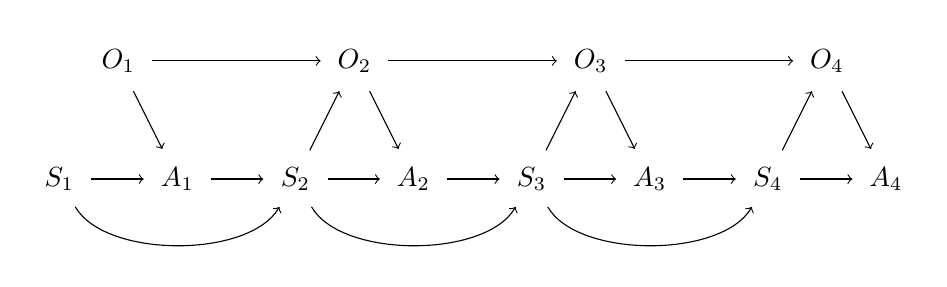
\begin{tikzpicture}
        \foreach \i in {1,2,3,4}{
            \node[circle,
                minimum size=5mm] (o-\i) at (3*\i-0.75,1.5) {$O_\i$};}
        \foreach \i in {1,2,3,4}{
            \node[circle, 
                minimum size=5mm] (a-\i) at (3*\i,0) {$A_\i$};}
        \foreach \i in {1,2,3,4}{
            \node[circle, 
                minimum size=5mm] (s-\i) at (3*\i-1.5,0) {$S_\i$};}
        \foreach \i in {1,2,3,4}{
            \draw[->] (s-\i) -- (a-\i);
            \draw[->] (o-\i) -- (a-\i);}
        \foreach \i in {2,3,4}{
            \draw[->] (s-\i) -- (o-\i);}
        \foreach \i [evaluate=\i as \j using {int(\i+1)}] in {1,2,3}{
            \draw[->] (o-\i) -- (o-\j);}
        \foreach \i [evaluate=\i as \j using {int(\i+1)}] in {1,2,3}{
            \draw[->] (a-\i) -- (s-\j);
            \path (s-\i) edge[out=-60,in=-120,looseness=0.75,->] (s-\j);}
    \end{tikzpicture}}
    \caption{Bayesian network of the HRL option framework.}
    \label{fig:Bayes_net}
\end{figure}

\subsection{The HIL Problem}

Suppose that an expert uses the HRL with options framework to generate a sequence of states and actions $\{(s_t,a_t)\}_{t = 1}^T$.
In the HIL problem, we seek to use this sequence to learn the expert's underlying low and high-level policies $\pi_{lo}$ and $\pi_{hi}$.
The associated options $\{o_t\}_{t = 1}^T$ are not observed and constitute hidden (or latent) variables.
The HIL problem is thus an instance of learning in the presence of latent variables which has motivated its solution via EM approaches in \citep{Daniel2016,zhiyu20,Giammarino_2021}.
Due to local convergence issues inherent in EM approaches, we shall take a different approach and develop a method of moments for HIL inspired by the method of moments for HMMs developed in \citep{hsu08}.

To develop our method, we define the following matrices.
\begin{definition}
    For $s \in \mathcal{S}$, define $\bm{\Pi}^{lo}_s\in\mathbb{R}^{\omega\times\alpha}$ with $$\bm{\Pi}^{lo}_s[o,a] = \pi_{lo}(A_t=a\vert O_t=o,S_t=s)$$ as the matrix representation of $\pi_{lo}$ under the state $s$.
\end{definition}

\begin{definition}
    For $s \in \mathcal{S}$, define $\bm{\Pi}^{hi}_s\in\mathbb{R}^{\omega\times\omega}$ with $$\bm{\Pi}^{hi}_s[o,o'] = \pi_{hi}(O_{t+1} = o'\vert O_t = o,S_{t+1}=s)$$
    as the matrix representation of $\pi_{hi}$ under the state $s$.
\end{definition}

\begin{definition}
    For $a \in \mathcal{A}$, define $\bm{\Phi}^A_a\in\mathbb{R}^{\zeta\times\zeta}$ with
    \[
        \bm{\Phi}^A_a[s,s']=\Phi(S_{t+1} = s'\vert S_t = s, A_t=a)
    \]
    as matrix representations of the transition dynamics.
\end{definition}

\begin{definition}
    For $s'\in\mathcal{S}$, define $\bm{\Xi}_{s'}\in\mathbb{R}^{\zeta\times\omega}$ with $$\bm{\Xi}_{s'}[s,o] = P(S_t=s,O_t=o,S_{t+1}=s').$$
\end{definition}

We also require the following mild regulatory assumptions.
\begin{assumption}[Option-Action Identifiability]\label{asu:pilo}
Under the same state, no two options contain the same policy for choosing an action, i.e., $\bm{\Pi}^{lo}_s$ has full row rank $\forall s\in\mathcal{S}$.
\end{assumption}

\begin{assumption}[Option-Option Identifiability]\label{asu:pihi}
Under the same state, no two options give the same policy for choosing the next option, i.e., $\bm{\Pi}^{hi}_s$ has full rank $\forall s\in\mathcal{S}$. 
\end{assumption}

\begin{assumption}\label{asu:invertibility}
$\bm{\Xi}_s$ has full column rank $\forall s\in\mathcal{S}$.
\end{assumption}

\begin{assumption}\label{asu:noisy_transition}
All actions have a non-zero chance of transitioning a state to all of its neighboring states and one state is another state's neighbor if there exists an action under which the probability of transitioning from the latter to the former is non-zero, i.e., for any $s,s'\in\mathcal{S}$, if there exists $a\in\mathcal{A}$ such that $\bm{\Phi}^A_a[s,s']>0$, then $\bm{\Phi}^A_{a'}[s,s']>0,\forall a'\in\mathcal{A}.$
\end{assumption}

\begin{assumption}[Stationary]\label{asu:stationary}
The process $(O_t,S_t)$ starts with the stationary distribution, that is $\bm{\pi}^1_s[o]=\bm{\pi}^\infty_s[o]$ where $\bm{\pi}^t_s\in\mathbb{R}^\omega$ with $\bm{\pi}^t_s[o]=P(O_t=o,s_t=s)$ for $s \in \mathcal{S}$.
\end{assumption}
\begin{remark}
Assumptions \ref{asu:pilo}, \ref{asu:pihi}, and \ref{asu:invertibility} follow the same line of reasoning as Condition 1 of \cite{hsu08}; they remove malicious instances that can cause learning to confuse options that have the same transition/action probability. Assumption \ref{asu:noisy_transition} is needed as the method of moments relies on the cancellation of certain terms across all actions, it can be interpreted as an action emission noise in the expert or a transition noise in the environment.
\end{remark}
% \npnguyen{Assumption \ref{asu:invertibility} can be dropped at the cost of increasing the size of the matrix $M$ from $\zeta\zeta\times\zeta\alpha$ to $\zeta\zeta\alpha\times\zeta\alpha$. What is your opinion?}

\section{Spectral method of moments}

In this section, we develop our method of moments for HIL.
We specifically identify observable moments of the states and actions, and show that they enable recovery of the low-policy $\pi_{lo}$ via matrix diagonalization and the high-level policy $\pi_{hi}$ via simple matrix algebra.

\subsection{Moments in HIL}
We note that under Assumption \ref{asu:stationary}, the moments of the states, options, and actions are time-invariant.
Thus, without loss of generality, we consider the moments $\bm{M}_a\in \mathbb{R}^{\zeta\zeta\times\zeta\alpha}$ for $a\in\mathcal{A}$ with
\[
    &\bm{M}_a\lrb{s_2\zeta+s_1,s_3\alpha+a_3}\\
        &\quad=\ P(S_2=s_2,S_1=s_1,A_2=a,S_3=s_3,A_3=a_3),
      %  \numberthis
\]
and $\bm{K}_{s}\in\mathbb{R}^{\zeta\times\alpha}$ for $s\in\mathcal{S}$ with
\[
    \bm{K}_s[s_1,a_2]
    = P(S_1=s_1,S_2=s,A_2=a_2). %\numberthis
\]
Our goal now is to construct an expression of these observable moments that allows the recovery of the low-level policy via matrix diagonalization.

\subsection{Diagonalizable Forms}

We first examine the properties of $\bm{K}_s$ for $s \in \mathcal{S}$.
Specifically, let $\bm{V}_s\in\mathbb{R}^{\alpha\times\omega}$ for $s \in \mathcal{S}$ be a matrix of right singular vectors corresponding to the $\omega$ largest singular values of $\bm{K}_s$.
We then have the following lemma.
%Finally, the proof of the core theorem makes use of the following lemma:
\begin{lemma}%[Action Projection invertibility]
\label{lem:actionProjection}
Define the block-diagonal matrices
\[\label{eq:Vmat}
    \bm{V} = \bmat{\bm{V}_1&&\\&\ddots&\\&&\bm{V}_\zeta} \text{ and } \bm{\Pi}^{lo}=\bmat{\bm{\Pi}^{lo}_1&&\\&\ddots&\\&&\bm{\Pi}^{lo}_\zeta}.
\]
Then the product matrix
\[
    \bm{\Pi}^{lo}\bm{V} = \bmat{\bm{\Pi}^{lo}_1\bm{V}_1&&\\&\ddots&\\&&\bm{\Pi}^{lo}_\zeta\bm{V}_\zeta}
\]
is invertible.
\end{lemma}
\begin{proof}
We have
\[
    \bm{K}_s[s_1,a_2]
    %=&P(S_1=s_1,S_2=s,A_2=a_2)\\
    &=\sum_{o_1}\sum_{o_2} P(O_1=o_1,S_1=s_1,S_2=s)\\
    &\qquad\times \pi_{hi}(O_2=o_2\vert O_1=o_1,S_2=s)\\
    &\qquad\times \pi_{lo}(A_2=a_2\vert O_2=o_2,S_2=s)\\
    &=\lrc{\bm{\Xi}_s\bm{\Pi}^{hi}_s\bm{\Pi}^{lo}_s}[s_1,a_2].\label{eq:overline_K_derive}
\]

This implies $\mathrm{rowspan}(\bm{K}_s)\subseteq\mathrm{rowspan}(\bm{\Pi}^{lo}_s)$. In addition, because $\bm{\Xi}_s$ is full column rank and $\bm{\Pi}^{hi}_s$ is full rank (Assumptions \ref{asu:pihi} and \ref{asu:invertibility}),
\[
    \bm{\Pi}^{lo}_s=(\bm{\Xi}_s\bm{\Pi}^{hi}_s)^+\bm{K}_s,
\]
which implies $\mathrm{rowspan}(\bm{\Pi}^{lo}_s)\subseteq\mathrm{rowspan}(\bm{K}_s)$. Thus,
\[
    \mathrm{rowspan}(\bm{V}_s\transpose)
        =\mathrm{rowspan}(\bm{K}_s)
        =\mathrm{rowspan}(\bm{\Pi}^{lo}_s).
\]
Therefore, $\bm{\Pi}^{lo}_s\bm{V}_s$ is invertible. Since $s$ is chosen arbitrarily, this applies for all $s$.
% Now consider
% \[
%     \bm{\Pi}^{lo}\bm{V} = \bmat{\bm{\Pi}^{lo}_1\bm{V}_1&&\\&\ddots&\\&&\bm{\Pi}^{lo}_\zeta\bm{V}_\zeta}.
% \]
Because $\bm{\Pi}^{lo}_s\bm{V}_s$ is invertible for all $s$, it follows that $\bm{\Pi}^{lo}\bm{V}$ is also invertible.
\hspace*{\fill} \qed
\end{proof}

We next examine the properties of the moments $\bm{M}_a$.
Before doing so, note that the moments $\bm{M}_a$ involve the transition dynamics $\bm{\Phi}^A_a$ as well as the underlying low- and high-level policies we are interested in. 
To remove the influence of the transition dynamics on $\bm{M}_a$, let us define the kernel matrix $\bm{\Psi} \in \mathbb{R}^{\zeta \times \zeta}$ with
\[
    \bm{\Psi}[s_2,s_3]&=\left\{\begin{aligned}\label{eq:psi}
        &\psi_{s_2s_3},\quad&\text{if}\ \bm{\Phi}^A_a[s_2,s_3]>0\ \forall a\in\mathcal{A},\\
        &0,\quad&\text{otherwise},
    \end{aligned}\right.
\]
and normalizer matrices $\bm{N}_a \in \mathbb{R}^{\zeta \times \zeta}$ for $a \in \mathcal{A}$ with
\[
    \bm{N}_a[s_2,s_3]&=\left\{\begin{aligned}\label{eq:normmat}
        &\frac{1}{\bm{\Phi}^A_a[s_2,s_3]},\quad&\text{if}\ \bm{\Phi}^A_a[s_2,s_3]>0,\\
        &0,\quad&\text{otherwise,}
    \end{aligned}\right.
\]
where $\psi_{s_2s_3}$ are constants of choice such that $\bm{\Psi}$ is full rank (such constants will always exist under Assumption \ref{asu:noisy_transition}). %Choosing these constants so as to minimize the sample complexity will be reserved for future works.
We then may define the surrogate moments
\[\label{eq:mathcalM}
    \bm{\hat{M}}_a = (\bm{\Psi}\otimes\one_{\zeta\times\alpha})\circ (\bm{N}_a\otimes\one_{\zeta\times\alpha})\circ \bm{M}_a,
\]
for $a \in \mathcal{A}$ and 
\[\label{eq:mathcalM_sum}
    \bm{\hat{M}} = \sum_{a\in\mathcal{A}}\bm{\hat{M}}_a
\]
that do not depend on the transition dynamics where $\bm{\hat{M}}_a$ and $\bm{\hat{M}}$ have the same dimensions as $\bm{M}_a$.

These surrogate moments combined with Lemma \ref{lem:actionProjection} lead to the following theorem that establishes that the observable moments allow the recovery of the low-level policy via matrix diagonalization.
\begin{theorem}\label{theo:central}
The product $\bm{V}\transpose\bm{\hat{M}}^+\bm{\hat{M}}_a\bm{V}$ admits the factorization:
\[\label{eq:diagonalize}
    \bm{V}\transpose\bm{\hat{M}}^+\bm{\hat{M}}_a\bm{V} = \bm{B}\inv\bm{\Lambda}_a\bm{B},
\]
where
\[\label{eq:Lambda_definition}
    \bm{\Lambda}_a = \bmat{\mathrm{diag}(\bm{\Pi}^{lo}_1\unit_a)&&\\
              &\ddots&\\
              &&\mathrm{diag}(\bm{\Pi}^{lo}_{\zeta}\unit_a)}.
\]
\end{theorem}
\begin{proof}
% Let us define
% \[
%     \bm{\Xi}\lrb{s_2\zeta+s_1, s_2'\omega+o_1}
%     &=\ P(O_1=o_1,S_1=s_1,S_2=s_2=s_2')\notag\\
%     &=\ \begin{cases}
%             \bm{\Xi}_{s_2}[s_1,o_1]\ &\text{if}\ s_2=s_2'\\
%             0\ &\text{otherwise}.
%         \end{cases}
% \]
Let 
\[
    \bm{\Xi}=\bmat{\bm{\Xi}_1&&\\&\ddots&\\&&\bm{\Xi}_\zeta}
    \text{ and } \bm{\Pi}^{hi}=\bmat{\bm{\Pi}^{hi}_1&&\\&\ddots&\\&&\bm{\Pi}^{hi}_\zeta}.
\]
% Next, we define
% \[
%     &\bm{\Pi}^{lo}[s_1\omega+o_1,s_1'\alpha+a_1]\\
%     =\ &\pi_{lo}(A_1=a_1,S_1=s_1'\vert O_1=o_1,S_1=s_1)\\
%     =\ &\left\{\begin{aligned}
%         &\bm{\Pi}^{lo}_{s_1}[o_1,a_1]\ &\text{if}\ s_1=s_1'\\
%         &0\ &\text{otherwise}
%     \end{aligned}\right. ,\numberthis
% \]
% \[
%     &\bm{\Pi}^{hi}[s_2\omega+o_1,s_2'\omega+o_2]\\
%     =\ &\pi_{hi}(O_2=o_2,S_2=s_2'\vert O_1=o_1,S_2=s_2)\\
%     =\ &\left\{\begin{aligned}
%         &\bm{\Pi}^{hi}_{s_2}[o_1,o2]\ &\text{if}\ s_2=s_2'\\
%         &0\ &\text{otherwise}
%     \end{aligned}\right. .\numberthis
% \]

% As defined in \eqref{eq:Lambda_definition},
% \[
%     \bm{\Lambda}_a = \bmat{\mathrm{diag}(\bm{\Pi}^{lo}_1\unit_a)&&\\
%               &\ddots&\\
%               &&\mathrm{diag}(\bm{\Pi}^{lo}_{\zeta}\unit_a)}.
% \]

% The entries of $\bm{\Lambda}_a$ can be interpreted as
% \begin{multline}
%     \bm{\Lambda}_a[s_t\omega+o_t,s_t'\omega+o_t']\\
%     =\pi_{lo}(A_1=a_1,S_t=s_1',O_1=o_1'\vert O_1=o_1,S_t=s_1)
% \end{multline}
Then,
\[
  &\bm{M}_a\lrb{s_2\zeta+s_1,s_3\alpha+a_3}\\
  %=\ &P(S_2=s_2,S_1=s_1,A_2=a,S_3=s_3,A_3=a_3)\\
  =\ &\sum_{s_2',o_1}
      \sum_{s_2'',o_2}
      \sum_{s_2''', o_2'}
      \sum_{s_3, o_2'}
      \sum_{s_3', o_2''}\\
  &\qquad \phantom{\times}\ P(O_1=o_1,S_1=s_1,S_2=s_2=s_2')\\
  &\qquad \times\pi_{hi}(O_2=o_2,S_2=s_2''\vert O_1=o_1,S_2=s_2')\\
  &\qquad \times\pi_{lo}(A_2=a,S_2=s_2''',O_2=o_2'\vert O_2=o_2, S_2=s_2'')\\
  &\qquad \times P(S_3=s_3,O_2=o_2''\vert A_2=a,S_2=s_2''', O_2=o_2')\\
  &\qquad \times\pi_{hi}(O_3=o_3,S_3=s_3'\vert O_2=o_2'',S_3=s_3)\\
  &\qquad \times\pi_{lo}(A_3=a_3,S_3=s_3''\vert O_3=o_3,S_3=s_3')\\
  =\ &\lrc{\bm{\Xi}\bm{\Pi}^{hi}\bm{\Lambda}_a(\bm{\Phi}^A_a\otimes
      \identity_\omega)\bm{\Pi}^{hi}\bm{\Pi}^{lo}}
  \lrb{s_2\zeta+s_1,s_3\alpha+a_3}.%\numberthis
\]
Consider the $\zeta\times\alpha$ submatrix
\[
    \bm{U}^a_{s_2s_3}[s_1, a_3] &= 
        \bm{M}_a[s_2\zeta+s_1,s_3\alpha+a_3]\\
    \Leftrightarrow \bm{U}^a_{s_2s_3} &=
        \bm{\Xi}_{s_2}\bm{\Pi}^{hi}_{s_2}\mathrm{diag}(\bm{\Pi}^{lo}_{s_2}\unit_a)
        \bm{\Phi}^A_a[s_2,s_3]\bm{\Pi}^{hi}_{s_3}\bm{\Pi}^{lo}_{s_3}. %\numberthis
\]
Notice that $\bm{\Phi}^A_a[s_2,s_3]$ is a real number that can be estimated using observable data. We define
\[
    \bm{\hat{U}}^a_{s_2s_3} &= \frac{1}{\bm{\Phi}^A_a[s_2,s_3]}\bm{U}^a_{s_2s_3} \\
    &=\bm{\Xi}_{s_2}\bm{\Pi}^{hi}_{s_2}\mathrm{diag}(\bm{\Pi}^{lo}_{s_2}\unit_a)
        \bm{\Pi}^{hi}_{s_3}\bm{\Pi}^{lo}_{s_3} \label{eq:sub_mathcalM}
\]
 for all $s_2, s_3\in\mathcal{S}$ such that $\bm{\Phi}^A_a[s_2,s_3]>0, \forall a\in\mathcal{A}$, and $\bm{\hat{U}}^a_{s_2s_3} = \zero_{\zeta\times\alpha}$ otherwise.


By the Definitions (\ref{eq:mathcalM},~\ref{eq:sub_mathcalM})
\[
    \bm{\hat{M}}_a &=(\bm{\Psi}\otimes\one_{\zeta\times\alpha})\circ\bmat{\bm{\hat{U}}^a_{11}
        &\dots&\bm{\hat{U}}^a_{1\zeta}\\
    \vdots&\ddots&\vdots\\ \bm{\hat{U}}^a_{\zeta 1}&\dots&\bm{\hat{U}}^a_{\zeta\zeta}}\\
    &=\bm{\Xi}\bm{\Pi}^{hi}\bm{\Lambda}_a
        (\bm{\Psi}\otimes \identity_\omega)\bm{\Pi}^{hi}\bm{\Pi}^{lo}.%\numberthis
\]

By the Definition \eqref{eq:mathcalM_sum}
\[
    \bm{\hat{M}} &= \sum_{a\in\mathcal{A}}\bm{\hat{M}}_a\\
    &=\bm{\Xi}\bm{\Pi}^{hi}\lrp{\sum_{a\in\mathcal{A}}\bm{\Lambda}_a}
        (\bm{\Psi}\otimes \identity_\omega)\bm{\Pi}^{hi}\bm{\Pi}^{lo}\\
    &=\bm{\Xi}\bm{\Pi}^{hi}(\bm{\Psi}\otimes \identity_\omega)\bm{\Pi}^{hi}\bm{\Pi}^{lo}.%\numberthis
\]
Finally, we can write Equation \eqref{eq:diagonalize} as
\[
    &\bm{V}\transpose\bm{\hat{M}}^+\bm{\hat{M}}_a\bm{V}\\
    =&\lrp{\bm{\Pi}^{hi}\bm{\Pi}^{lo}\bm{V}}\inv
        \lrp{\bm{\Psi}\inv\otimes\identity_\omega}
        \bm{\Lambda}_a(\bm{\Psi}\otimes \identity_\omega)
        \bm{\Pi}^{hi}\bm{\Pi}^{lo}\bm{V},\label{eq:diagonalize_detailed}
\]
and the proof is complete.
\hspace*{\fill} \qed
\end{proof}

In order to compute the eigenbasis that jointly diagonalize \eqref{eq:diagonalize} for all $a\in\mathcal{A}$, we find a vector $\bm{\eta}\in\mathbb{R}^{\alpha}$ such that the eigenvalues of
\[\label{eq:jointDiag}
    \sum_{a\in\mathcal{A}}\bm{\eta}_a\bm{V}\transpose\bm{\hat{M}}^+\bm{\hat{M}}_a\bm{V}=
    \bm{B}\lrp{\sum_{a\in\mathcal{A}}\bm{\eta}_a\bm{\Lambda}_a}\bm{B}\inv
\]
are well spread. In other words, we find $\bm{\eta}$ such that the values $\unit_o\transpose\bm{\Pi}^{lo}_s\bm{\eta}$ are distinct and non-zero for all $(o,s)\in\mathcal{O}\times\mathcal{S}$. As suggested in \cite{HsuKakade13}, this can be satisfied in most cases if $\bm{\eta}$ is sampled uniformly from the surface of a unit sphere in $\mathbb{R}^\alpha$.

The eigen-decomposition will yield an eigenbasis up to a permutation $\bm{\mathcal{P}}\in\mathbb{R}^{\omega\times\zeta}$ of the pair $(o,s)\in\mathcal{O}\times\mathcal{S}$. To put it differently, the diagonal matrix obtained from diagonalizing $\bm{V}\transpose\bm{\hat{M}}^+\bm{\hat{M}}_a\bm{V}$ using this basis will be of the form
$\bm{\mathcal{P}}\bm{\Lambda}_a\bm{\mathcal{P}}\transpose$.
With some further processing, an order up to a permutation $\bm{\hat{\mathcal{P}}}\in\mathbb{R}^\omega$ of $o\in\mathcal{O}$ can be recovered, meaning the diagonal matrix obtained will be of the form $(\identity_\zeta\otimes\bm{\hat{\mathcal{P}}})\bm{\Lambda}_a(\identity_\zeta\otimes\bm{\hat{\mathcal{P}}}\transpose)$. This ordering corresponds to the relabeling of the options. Because this recovery process, while necessary, does not represent the main contribution of this work, it will be elaborated in the Appendix.

After obtaining the low-level policy matrices $\bm{\hat{\mathcal{P}}}\bm{\Pi}^{lo}_s$, the high-level policy matrices can be computed by the following theorem, up to the permutation $\bm{\hat{\mathcal{P}}}$ of the options.
\begin{theorem}
\[\label{eq:pihi_recovery}
    \bm{\hat{\mathcal{P}}}\bm{\Pi}^{hi}_{s'}\bm{\hat{\mathcal{P}}}\transpose=
        \sum_s \bm{w}_{s'}[s]\lrp{\bm{\hat{\mathcal{P}}}\bm{\Pi}^{lo}_s
        \bm{K}_s^+\bm{\hat{K}}_{ss'}
        {\bm{\Pi}^{lo}_{s'}}^+\bm{\hat{\mathcal{P}}}\transpose},
\]
where:
\begin{itemize}
    \item $\bm{\hat{K}}_{ss'}$ is a $\zeta\times\alpha$ submatrix of $\bm{\hat{M}}$ defined by
    \[\label{eq:hat_K_definition}\citep{Bauer:2007}
        \bm{\hat{K}}_{ss'}[s'',a]=\bm{\hat{M}}[s\zeta+s'',s'\alpha+a].
    \]
    \item $\bm{w}_{s'}$ are length $\zeta$ weight vectors of choice subject to
    \[\label{eq:pihi_weight_constraint}
        \bm{w}_i\transpose\bm{\Psi} \unit_i\transpose=1,\ \forall i\in\mathcal{S}.
    \]
\end{itemize}
\end{theorem}
\begin{proof}
According to Definition \eqref{eq:hat_K_definition} and Equation \eqref{eq:overline_K_derive}, $\bm{K}_s$ and $\bm{\hat{K}}_{ss'}$ can be written as following:
\[
    \bm{K}_s = \bm{\Xi}_s\bm{\Pi}^{hi}_s\bm{\Pi}^{lo}_s,
\]
\[
    \bm{\hat{K}}_{ss'} = \bm{\Psi}[s,s']\lrp{\bm{\Xi}_s\bm{\Pi}^{hi}_s\bm{\Pi}^{hi}_{s'}\bm{\Pi}^{lo}_{s'}}.
\]
Therefore,
\[
    &\bm{\Pi}^{lo}_s{\bm{K}_s}^+\bm{\hat{K}}_{ss'}{\bm{\Pi}^{lo}_{s'}}^+\\
    =\ &\bm{\Psi}[s,s']\lrp{\bm{\Pi}^{lo}_s{\bm{\Pi}^{lo}_s}^+{\bm{\Pi}^{hi}_s}\inv
        {\bm{\Xi}_s}^+\bm{\Xi}_s\bm{\Pi}^{hi}_s\bm{\Pi}^{hi}_{s'}\bm{\Pi}^{lo}_{s'}{\bm{\Pi}^{lo}_{s'}}^+}\\
    =\ &\bm{\Psi}[s,s']\bm{\Pi}^{hi}_{s'}.%\numberthis
\]
With that, we contract the left hand side of Equation \eqref{eq:pihi_recovery}
\[
    &\sum_s \bm{w}_{s'}[s]\lrp{\bm{\hat{\mathcal{P}}}\bm{\Pi}^{lo}_s\bm{K}_s^+\bm{\hat{K}}_{ss'}
        {\bm{\Pi}^{lo}_{s'}}^+\bm{\hat{\mathcal{P}}}\transpose}\\
    =&\sum_s \bm{w}_{s'}[s]\bm{\Psi}[s,s']\lrp{\bm{\hat{\mathcal{P}}}\bm{\Pi}^{hi}_{s'}
        \bm{\hat{\mathcal{P}}}\transpose}\\
    =&\bm{\hat{\mathcal{P}}}\bm{\Pi}^{hi}_{s'}{\bm{\hat{\mathcal{P}}}}\transpose.
    %\numberthis
\]
The last equality holds because we chose $\bm{w}_{s'}$ such that $\sum_s \bm{w}_{s'}[s]\bm{\Psi}[s,s']=1$. Analysis of the choice of $\bm{w}_{s'}$ will be reserved for future work.
\hspace*{\fill} \qed
\end{proof}

\subsection{Proposed Method of Moments for HIL}
Given the observed sequence $\{(s_t,a_t)\}_{t = 1}^T$, our method of moments to learn the policies $\pi_{lo}$ and $\pi_{hi}$ is:
\begin{enumerate}[leftmargin=2cm, label=Step \arabic*:]
    \item Estimate $\bm{M}_a$, $\bm{K}_s$, and $\bm{\Phi}^A_a$ from data via:
    \[
        &\bm{M}_a\lrb{s_2\zeta+s_1,s_3\alpha+a_3}\\
        =\ &\frac{\sum_{t=1}^{T-2}\indicator{s_t=s_1,s_{t+1}=s_2,a_{t+1}=a,s_{t+2}=s_3,a_{t+2}=a_3}}{T-2},
            %\numberthis 
            \\
        &\bm{K}_s\lrb{s_1,a_2}
        =\ \frac{\sum_{t=1}^{T-1}\indicator{s_t=s_1,s_{t+1}=s,a_{t+1}=a_2}}{T-1},
            %\numberthis
    \]
    \[
        \bm{\Phi}^A_a[s,s'] &= \frac{\sum_{t=1}^{T-1}\indicator{s_t=s, a_t=a, s_{t+1}=s'}}{\sum_{t=1}^{T-1}\indicator{s_t=s, a_t=a}}.
    \]
    \item Compute the surrogate moments $\bm{\hat{M}}_a$ and $\bm{\hat{M}}$ according to Equations \eqref{eq:mathcalM} and \eqref{eq:mathcalM_sum}.

    \item Perform SVD on $\bm{K}_s$, and construct the matrix $\bm{V}$ according to Equation \eqref{eq:Vmat}.
    \item Compute the joint eigenbasis $\bm{B}$ using Equation \eqref{eq:jointDiag}. Then, recover the order of its column using the algorithm discussed in the Appendix.
    \item Recover $\bm{\Pi}^{lo}$ using the diagonals that result from diagonalizations according to Equation \eqref{eq:diagonalize}.
    \item Compute $\bm{\Pi}^{hi}$ with Equation \eqref{eq:pihi_recovery}.
\end{enumerate}

\subsection{Performance discussion}
The algorithm consists of two parts, data collection with complexity $\mathcal{O}(T)$, and data processing with complexity $\mathcal{O}(\zeta^4\alpha\omega)$, dominated by the cost of computing $\bm{V}\transpose\bm{\hat{M}}^+\bm{\hat{M}}_a\bm{V}$ and its eigenbasis. This gives us the total time complexity of $\mathcal{O}(T+\zeta^4\alpha\omega)$.

Comparison to the EM methods presented in \cite{zhiyu20} and \cite{Giammarino_2021}, which has time complexity of $\mathcal{O}(T\omega^2)$ and $\mathcal{O}(\zeta\alpha\omega^3)$ per iteration respectively, can be difficult. This is due to the fact that they have different bottlenecks, along with the fact that the method of moments is parameter-less while EM methods need initialization. However, a general rule is that the larger the number of samples is relative to the number of states and actions, the better the method of moments performs compared to EM.

Another thing to note is that the techniques mentioned can be synergistic, with the output of the method of moments being good initialization for EM methods to refine.
\section{Experiment}
In this section, we examine the proposed algorithm in numerical experiments.
We will use a similar setup to \cite{zhiyu20} to test our model. Let there be a finite state machine with four states and the following parameters:
\[
    \bm{\Pi}^{hi}_1=\bmat{0.67&0.33\\0.16&0.84},\quad
    \bm{\Pi}^{hi}_2=\bmat{0.88&0.12\\0.16&0.84},\\
    \bm{\Pi}^{hi}_3=\bmat{0.84&0.16\\0.12&0.88},\quad
    \bm{\Pi}^{hi}_4=\bmat{0.84&0.16\\0.33&0.67}.%\numberthis
\]
\[
    \bm{\Pi}^{lo}_1=\bmat{0.6&0.4\\0.1&0.9},\quad
    \bm{\Pi}^{lo}_2=\bmat{0.7&0.3\\0.15&0.85},\\
    \bm{\Pi}^{lo}_3=\bmat{0.8&0.2\\0.3&0.7},\quad
    \bm{\Pi}^{lo}_4=\bmat{0.9&0.1\\0.35&0.65}.%\numberthis
\]
\[
    \bm{\Phi}^A_1=\bmat{0.7&0.1&0.1&0.1\\
        0.4&0.4&0.1&0.1\\0.3&0.3&0.3&0.1\\
        0.25&0.25&0.25&0.25},\\
    \bm{\Phi}^A_2=\bmat{0.25&0.25&0.25&0.25\\
        0.1&0.3&0.3&0.3\\0.1&0.1&0.4&0.4\\
        0.1&0.1&0.1&0.7}.%\numberthis
\]

The error will be measured by:
\[
    \mathrm{ERROR}=\sqrt{\norm{\bm{\Pi}^{lo}-\overline{\bm{\Pi}}^{lo}}^2_2
        +\norm{\bm{\Pi}^{hi}-\overline{\bm{\Pi}}^{hi}}^2_2},
\]
where $\overline{\bm{\Pi}}^{lo},\overline{\bm{\Pi}}^{hi}$ are the predicted values of $\bm{\Pi}^{lo},\bm{\Pi}^{hi}$.

For intuition, we can think of the states as locations on a number line (i.e., states with larger index are further right), the actions are $\mathcal{A}=\{\textrm{move-left},\textrm{move-right}\}$, and the options are $$\mathcal{O}=\{\textrm{tend-to-move-left},\textrm{tend-to-move-right}\}.$$ Looking at the numbers, we can see that the agent wants to alternately move from left to right and right to left.

\begin{figure}
    \centering
    \resizebox{0.4\textwidth}{!}{\begin{tikzpicture}
    \begin{loglogaxis}[
        width = 0.5\textwidth,
        height = 0.25\textwidth,
        xlabel = {$T$},
        ylabel = {$\mathrm{ERROR}$},]
     
    % Plot data from a file
    \addplot[
        thin,
        red,
    ] file[] {figures/sample_error.txt};
    \addplot[
        thin,
        blue,
    ] file[] {figures/sample_error_2.txt};
    \addplot[
        thin,
        green,
    ] file[] {figures/sample_error_3.txt};
     
    \end{loglogaxis}
 
    \end{tikzpicture}}
    \caption{Log-log plot of the error versus the number of sample points for several realizations of the problem.}
    \label{fig:error}
\end{figure}


In Fig.\ \ref{fig:error} we plot the error versus the number of samples for a few runs of our method in log scale. It can be seen that the error is polynomial relative to the number of samples.

For comparison purposes, Fig.\ \ref{fig:EM_error} depicts a few EM runs with randomized initialization and a sample size of $3 \times 10^5$. It can be seen that initialization have a significant effect on EM's rate of convergence and whether or not it arrives at the correct optima. In contrast, the proposed method of moments does not require initialization.
\begin{figure}
    \centering
    \resizebox{0.4\textwidth}{!}{\begin{tikzpicture}
    \begin{semilogyaxis}[
        width = 0.5\textwidth,
        height = 0.25\textwidth,
        xlabel = {Iterations},
        ylabel = {$\mathrm{ERROR}$},]
     
    % Plot data from a file
    \addplot[
        thin,
        red,
    ] file[] {figures/plot_2_0_300000.txt};
    \addplot[
        thin,
        green,
    ] file[] {figures/plot_2_1_300000.txt};
    \addplot[
        thin,
        blue,
    ] file[] {figures/plot_2_2_300000.txt};
    \addplot[
        thin,
        black,
    ] file[] {figures/plot_2_3_300000.txt};
    \addplot[
        thin,
        orange,
    ] file[] {figures/plot_2_4_300000.txt};
    \addplot[
        thin,
        cyan,
    ] file[] {figures/plot_2_5_300000.txt};
     
    \end{semilogyaxis}
 
    \end{tikzpicture}}
    \caption{Iterations versus error of EM runs with various initializations, some of which do not converge.}
    \label{fig:EM_error}
\end{figure}

\section{Conclusions and Future Work}
\label{sec:conclusions}
We developed a novel method of moments for Hierarchical Imitation Learning (HIL) that offers global convergence under mild regulatory conditions.
Our method of moments for HIL is based on similar methods for HMMs and other latent variable models, and avoids the local convergence issues inherent in previous Expectation-Maximization (EM) approaches to HIL.
Future work could include further relaxation of the conditions under which the method holds and examining its extension to situations in which the options form a semi-Markov (rather than a Markov) process.

\section{Introduction}
\label{sec:intro}

Characterizing latent structures with meaningful real-world interpretations is a central task in statistics.
In scientific applications, this task often amounts to discovering unobserved physical ``processes'' that generate observable quantities.
%To be concrete, consider two common classes of models aimed at the discovery of latent processes (although our setting and methods will be more general. 
For example, processes might correspond to subpopulations that cannot be directly observed such as
types of cells \citep{Gorsky:2020,Prabhakaran:2016}, behavioral genotypes \citep{Stevens:2019}, or
groups with canonical patterns of IQ development \citep{Bauer:2007}.
Also, processes could correspond to a variety of scientifically important objects such cell programs \citep{Kotliar_Identify_Cell_Idendity_Activity_NMF_2019,Buettner_FscLVM_ScalableVersatile_FA_2017,Risso_General_Flexible_Signal_Extract_2018},
mutational processes in tumors %(e.g., using whole genome sequencing data) 
\citep{Levitin_DeNovo_Gene_Signature_Identification_2019,Kinker_Pan_Cancer_2020,Seplyarskiy_PopulationSequencingData_2021},
or material types
\citep{Fevotte_NonlinearHyperspectralUnmixing_2015,Rajabi_SpectralUnmixingHyperspectral_2015}.

In practice, it is necessary to not only characterize each latent process but also determine \emph{how many} such processes there are.
This requires solving a model selection problem for a sequence of model families $\model{K} = \{ P_\theta : \theta \in \Theta_K\}$, $K = 1, 2, \dots,$ where $K$ denotes the number of latent processes in the model.
For example, $K$ could be the number of components in a mixture model or the number of factors in a factor analysis model.
Given some observed data $\data{1},\dots, \data{N} \distiid P_o$ that were generated by the output of $K_{o}$ latent processes,
the goal is to recover $K_{o}$ and a model $\widetilde{P}_o \in \model{K_{o}}$ such that $\widetilde{P}_o  \approx P_{o}$.
Standard frequentist and Bayesian model selection methods provide consistent estimation of $K_o$ when $\model{K_o}$ is \emph{well-specified} (that is, $P_o \in \model{K_o}$ but $P_o \notin \model{K}$ if $K < K_o$).
However, if $\model{K_o}$ is \emph{misspecified} (that is, $P_o \notin \model{K_o}$), then standard methods do not work as intended
\citep{Cai:2021,Guha:2021,Fruhwurth:2006,Miller:2019,Xue:2024}.
The reason for this failure is that these methods optimize for some measure of \emph{predictive performance} (e.g., some form of expected log loss).
Therefore, as $N \to \infty$, these methods will select a sequence of models that converge to the distribution $P_\star
	\in \model{\infty} = \bigcup_{K=1}^\infty \model{k}$ that has minimal Kullback--Leibler divergence between $P_o$ and all $P \in \model{\infty}$.
Since typically $P_\star \notin \model{K}$ for any finite $K$, when using a predictive method for
model selection, as the number of observations $N$ increases, rather than obtaining better estimates, the opposite occurs:
the distribution $P_o$ is better estimated by adding spurious latent structures that compensate for the shortcomings of the parametric model.
This problem is known as \emph{overfitting}  \citep{Cai:2021}. %

However, when trying discover real-world processes, the statistical problem is no longer predictive in nature, but rather \emph{explanatory}  \citep{Shmueli:2010}.
The aim is to infer meaningful constructs that capture the underlying causal structure 
-- in this case the latent processes -- even if doing so results in a fitted model with reduced
predictive power.
Hence, there is a need for robust model selection procedures that can replace current defaults such as the Akaike, Bayesian, and deviance information criteria \citep{Akaike:1974,Schwarz:1978,Spiegelhalter:2002}, which remain widely used due to their simplicity and the ease with
which they can be incorporated into data analysis workflows -- for example, when a user wants to use an existing (perhaps specialized) method to estimate the parameters of each model $\model{K}$ ($K = 1, 2, \dots$).
We defer a more detailed discussion of related work until after we describe 
out methodology. 


\paragraph{Contributions.}
In this paper, we make the following contributions to the development of more reliable
and robust methods for model selection for discovering real-world latent processes:
%overcome the limitations of existing approaches:
\begin{enumerate}
	%	\item We define a broad class of generative models (\cref{sec:motivation}) .
	%	      The key modeling assumption is that each latent process generates independent latent data for each observation;
	%	      the latent data from the processes are then combined to produce the observed data.
	%	      The class includes mixture models and factor models as special cases.
    \item We define a formal notion of \textit{robust model selection consistency}
    and argue that it captures key features any robust model selection method 
    should satisfy. 
	\item We propose the \emph{accumulated cutoff discrepancy criterion} (\methodname), as a simple, flexible approach to robust model selection. 
	\item We show how to apply \methodname to a broad class of models
	in which the observations are determined by combining (unobserved) outputs from $K$ latent processes.
	% \methodname combines ideas from minimum distance estimation and coarsening, and
	% can incorporate expert and prior knowledge about the nature of the model misspecification.
	%       \methodname can be used with any parameter estimation technique, so it is easy to incorporate
	      % into existing data analysis workflows. % (see \cref{sec:case-study} for a comprehensive illustration of this).
	      %      Our minimum distance approach enables the use of any discrepancy measure between distributions,
	      %     which can be chosen in an application-specific manner.
	      %    Given fitted models each possible number of components, the computational cost required to compute our criterion is determined by the cost of estimating the discrepancy measure, which is typically quite small.
	\item We prove that \methodname provides robust model selection 
    consistency for mixture models and probabilistic matrix factorization models, including factor analysis models. 
	      %for our model class (\cref{sec:motivation}).
	      %   We show that, under intuitive assumptions, our procedure is robustly consistent (\cref{sec:theory}), 
	      % as illustrated in the third row of \cref{fig:motivate-comparison}.
	\item We demonstrate the broad utility of \methodname through four numerical experiments using mixture and matrix factorization models
	      applied to simulated and real data.\footnote{Code to reproduce all experiments is available on GitHub: \url{https://github.com/TARPS-group/robust-model-selection-for-discovery}.} % (\cref{sec:experiments}).
	      % Experiments include cell type discovery using flow cytometry data and mutational process discovery using Poisson nonnegative matrix factorization.
	      We also provide an in-depth case study that shows our criterion provides state-of-the-art clustering accuracy of single-cell RNA-seq gene expression data.
          % ~(\cref{sec:case-study})
	% \item We conclude in \cref{sec:discussion} with a discussion of some limitations of our approach and directions for future work.
\end{enumerate}



\section{Methodology}
\label{sec:methods}

We first define robust model selection consistency, which naturally 
leads to a plug-in procedure, the accumulated cutoff discrepancy criterion (\methodname). 
We then describe how to apply \methodname for a broad class of latent
variable models.
In this section, we use mixture modeling as a running example to illustrate ideas. 
Let $\mcF = \{ F_{\phi} \mid \phi \in \Phi \}$ denote the component distribution family
and let $\eta \in \Delta_{\numcomps}$ denote the component weights, 
where $\Delta_\numcomps = \{ \eta \in \reals_{+}^{\numcomps} \mid \sum_{k=1}^{\numcomps} \eta_{k} = 1 \}$ 
is the $(\numcomps-1)$-dimensional probability simplex. 
Denote the parameter set for the $\numcomps$-component mixture distributions by 
$\Theta^{(\numcomps)} = \Delta_{\numcomps} \times \Phi^{\numcomps}$, so the 
mixture model distribution family is 
\[
\model{K} = \textstyle \left\{ P_\theta = \sum_{k=1}^K \eta_k F_{\phi_k} : \theta = (\eta, \phi_1,\dots,\phi_K) \in \Theta^{(\numcomps)}\right\}. 
\]
Recall that we can also write the generative process of the mixture model in terms of
latent variables $z_{n} \in \{1,\dots,K\}$ that indicate which component observation $n$ belongs to:
\[
z_n \mid \theta &\distas \distCat(\eta) &
x_n \mid z_n = k, \theta &\distas F_{\phi_{k}}. 
\]
Since we are interested in isolating contribution of each component, it is this latent variable
representation that will be most relevant. 
We discuss applications to other models in \cref{sec:framework,sec:pmf-applications}.

\subsection{Robust Model Selection Consistency} \label{sec:robust-consistency}

Generalizing the mixture model setting, consider a sequence of models $\model{1}, \model{2}, \dots, \model{K}, \dots$, where $K$ captures how many distinct latent components are generating the observed data.
Assume that $\model{K} = \{ P_{\theta} \mid \theta \in \paramSpace{K} \}$, where $\paramSpace{K}$ is the parameter space
and $P_{\theta} \in \mcP(\mathbb{X})$, the space of probability measures on the observation space $\mathbb{X}$. 
The objective is to identify the true number of processes $K_o$.
% as well as a model $P_\star \in \model{K_o}$ that fits the data well.
Fix a \emph{distribution-level discrepancy} $\distDisc$ on probability measures that will quantify the fit between $P_{\theta}$ and the data-generating distribution $P_{o}$.
We do not assume a unique minimizing parameter since, at the very least, 
the component indices in latent variable models are non-identifiable. 
Let $\Theta_{\star}^{(K)}(P_{o}) \defas \argmin_{\theta \in\paramSpace{K}} \distDisc(P_{o} \mid P_{\theta})$ 
denote the set of minimizing parameters.
Alternatively, a practitioner might choose a parameter estimation procedure that is not model-based, in which case it might converge to a parameter value in some other set, which we also denote by $\Theta_{\star}^{(K)}(P_{o})$.
%We will formally define robust model selection consistency in terms of the set-valued function $\Theta_{\star}(P_{o}, K) \defas \Theta_{\star}^{(K)}(P_{o})$. 

The challenge in the misspecified setting is that for any $\theta_{\star}^{(K)} \in \Theta_{\star}^{(K)}(P_{o})$, typically $\distDisc(P_{o} \mid P_{\theta_{\star}^{(K)}})$ is not minimized at $K = K_{o}$.
In fact, in our settings of interest $\model{K} \subsetneq \model{K+1}$ but $P_{o} \notin \model{K}$ for any $K$, so
$\distDisc(P_{o} \mid P_{\theta_{\star}^{(K)}})$ is monotonically decreasing as $K$ increases. 
To correctly recover $K_{o}$, the user must specify how much $P_{\theta}$ can deviate from $P_{o}$ while remaining an acceptable approximation.
Therefore, we introduce a second discrepancy which measures how well the \emph{components} of $P_{o}$ and $P_{\theta}$ match.
%deviates from the assumed model and allow for some positive degree of discrepancy. 

Since the components of $P_{o}$ are unknown, the component contributions must be estimated based on model $P_{\theta}$ but 
using the distribution of data from $P_{o}$. 
Let the \emph{component-level realized discrepancy} $\compDisc^{(K)}(\theta, k, P_{o})$ quantify
how close the inferred component $k \in \{1,\dots,K\}$ from $P_{o}$ is to component $k$ of the model
$P_{\theta}^{(K)}$. 
To quantify the overall degree of component-level misspecification of $P_o$ with true number of components $K_o$,
%for a fixed choice of inference algorithm, 
define the \emph{worst-case component-wise discrepancy}
\[
 \rho(P_{o}, K_{o}) \defas  \sup_{\theta \in \Theta_{\star}^{(K_{o})}(P_{o})} \max_{k \in [K_{o}]} \compDisc^{(K_{o})}(\theta, k, P_{o}).
\]
For example, in the mixture model case we can construct a component-level realized discrepancy by inferring
the component of $P_o$ that would correspond to each mixture component.
That is, if we assign each observation from $P_o$ according to the conditional component probabilities 
$p(k \mid x, \theta) = \eta_{k} \frac{\dee F_{\phi_k}}{\dee P_{\theta}}(x)$, 
then the inferred $k$th component of $P_o$ is 
\begin{align}
	\widetilde{F}^{(\theta)}_{ok} = \frac{p(k \mid x, \theta)}{\int p(k \mid y, \theta) P_o(\dee y)} P_o. 
\end{align}
Given a choice discrepancy measure $\mcD$ (e.g., $\distDisc$), we can set 
$
\compDisc^{(K)}(\theta, k, P_{o}) = \mcD(\widetilde{F}^{(\theta)}_{ok} \mid F_{\phi_k}).
$

\begin{definition}[Robust model selection consistency] \label{def:robust-consistency}
	Fix a function $\kappa : \reals_{+} \times \nats \to \reals_{+}$. 
	A model selection procedure $\widehat K(\data{1:N}, \rho) \in \nats$ is \emph{$\kappa$-robustly consistent for $\Theta_{\star}$ and $\compDisc$} if,
	for any data-generating distribution $P_o$ and true component number $K_o$ that satisfies 
	\[ \label{eq:mismatch-condition}
		\inf_{\theta \in \Theta_{\star}^{(K)}(P_{o})} \distDisc(P_{o} \mid P_{\theta}) \ge \kappa(\rho(P_{o}, K_{o}), K)
		\quad\text{for all $K \in \{1,\dots,K_{o}-1\}$},
	\]
	it holds that, for $\data{1}, \data{2}, \dots \distiid P_{o}$, 
	\[
		\Pr\big\{\widehat K(\data{1:N}, \rho(P_{o}, K_{o})) = K_o \big\} \overset{N \to \infty}{\longrightarrow} 1.
	\]
\end{definition}
%The model selection rule can depend on $\rho =  \rho(P_{o}, K_{o})$ since $\rho$ is not inferable using samples from $P_{o}$.
To interpret \cref{def:robust-consistency} and the role of the function $\kappa$, 
it is helpful to compare robust model selection consistency to classical model selection consistency.
\Cref{fig:consistency-illustration} provides a cartoon illustration of the differences between the two types of consistency. 
Classical model consistency typically requires that  
(1) $P_o \in \model{K_o}$ and (2) $P_{o} \notin \model{K}$ for $K < K_o$ \PROBLEM{add citations}.
Robust consistency weakens the first condition by allowing for a worst-case discrepancy $\rho(P_{o}, K_{o}) \ne 0$,
whereas classical consistency would require $\rho(P_{o}, K_{o}) = 0$.
However, robust consistency strengthens the second second by requiring a gap between $P_o$ 
and all models for $K < K_o$.
The size of this gap specified in \cref{eq:mismatch-condition} in terms of $\kappa$. 
Hence, we call $\kappa$ the \emph{gap function}. 
It would be natural to ask that $\kappa(\rho, K) = \rho$, although this may not always be possible. 

\begin{figure}[tp]
	\centering
	\includegraphics[width=.7\textwidth,trim=0in 6.2in 6.2in 0in,clip]{consistency-illustration}
	\caption{Cartoon illustration of the differences between traditional and robust model selection consistency
		where the true model corresponds to $K_{o} = 4$, with the nested models indicated by the gray ovals.
		We contrast five possible data-generating distributions, $P_{o}^{A}, \dots, P_{o}^{E}$, indicated by
		the gold points.
		Since $P_{o}^{A}, P_{o}^{B} \in \model{K_{o}}$ but are not in $\model{K}$ for $K < K_o = 4$,
		for these models $K_{o}$ can be consistently estimated.
		However,  since $P_{o}^{C}, P_{o}^{D}, P_{o}^{E} \notin \model{K_{o}}$, for these distributions
		$K_{o}$ cannot be estimated consistently in the traditional sense.
		On the other hand $P_{o}^{A}, P_{o}^{B}, P_{o}^{C}$, and $P_{o}^{D}$
		are close to $\model{K_{o}}$,
		so $K_{o}$ could potentially be robustly and consistently estimated in these four cases.
		However, $P_{o}^{B}$ and $P_{o}^{D}$ are also close to $\model{3}$, so robustly consistent
		estimation of $K_{o}$ is feasible only for $P_{o}^{A}$ and $P_{o}^{C}$.
		Since $P_{o}^{E}$ is far from $\model{K_{o}}$, $K_{o}$ would not be consistently estimable --
		either in the traditional or robust sense.
	}
	\label{fig:consistency-illustration}
\end{figure}



\subsection{A Plug-in Procedure}
\label{sec:method}

We propose a simple plug-in procedure for model selection, inspired by \cref{def:robust-consistency}.
Assuming $\rho_o = \rho(P_o, K_o)$ were known, we would want to find the smallest value of $K$ such that 
for all $k \in \{1,\dots,K\}$, we have $\compDisc^{(K)}(\theta_\star, k, P_{o}) \le \rho$ for $\theta_\star \in \Theta_{\star}^{(K_{o})}(P_{o})$.
However, since $P_{o}$ and $\Theta_{\star}^{(K_{o})}(P_{o})$ are unavailable, we propose to instead 
use the empirical distribution $\widehat{P}_o = \numobs^{-1} \sum_{n=1}^N \delta_{x_n}$, where $\delta_x$
is the Dirac measure at $x$, and a point estimator $\widehat\theta^{(K)}$.
Hence, we obtain the plug-in estimator $\compDiscEst^{(K,k)} = \compDisc^{(K)}(\widehat\theta^{(K)}, k, \widehat{P}_o)$.
Since values of $\compDiscEst^{(K,k)} < \rho_o$ are not important from a model selection perspective, 
we truncate the estimator by replacing it with $\max(0, \compDiscEst^{(K,k)} - \rho)$, where $\rho$ is 
a best estimate of $\rho_o$. 
We can view taking this maximum as serving a similar role to how the coarsened posterior conditions on the discrepancy having a known upper bound. 

Rather than taking the maximum over the component-wise discrepancy estimates, for better robustness
to noisy estimates we use a sum, which results in a robust model selection loss 
\[ \label{eq:robust-loss}
	\mathcal{R}^\rho(x_{1:n}, K) = \sum_{k=1}^K \max(0, \compDiscEst^{(K,k)} - \rho),
\]
where for notational simplicity we have left the dependence of $\compDiscEst^{(K,k)}$ on $x_{1:n}$ 
(as a function of $\widehat{P}_o$ and $\widehat\theta^{(K)}$) implicit. 
Since the loss is the sum (i.e., accumulation) of discrepancies that have been truncated (i.e., cut off) at $\rho$,
we call \cref{eq:robust-loss} the \emph{accumulated cutoff discrepancy criterion} (\methodname).
The corresponding robust model estimator is
\[
\widehat{K}^\rho(x_{1:n}) = \min\{\argmin_K \mathcal{R}^\rho(x_{1:n}, K)\}.
\]
Since $\argmin_{\numcomps}$ may return a set of values if the loss is equal to
zero for more than one value of $\numcomps$, it is necessary to include an
additional $\min$ operation to select the smallest value from the set.
We will discuss how to determine $\rho$ in \cref{sec:choosing-rho}. 

\subsection{Modeling Framework} \label{sec:framework}

\begin{figure}[tp]
	\centering
	\includegraphics[width=.8\textwidth,trim=0in 1.9in 0in 0in,clip]{model}
	\caption{Graphical representation of the general form for model $\model{K}$ for a single observation $\data{n}$.
		Circles denote random variables while squares denote deterministic variables.
		A gray background indicates global parameters while a black background indicates an observed quantity.}
	\label{fig:model}
\end{figure}

Guaranteeing robust model consistency requires specific choices of model and component-level discrepancy.
In this paper, we consider a flexible modeling framework in which the observed data are the result of $K$ distinct latent sources (\cref{fig:model}). 
This framework will lead to a natural choice of component-level discrepancy, of which the mixture model
discrepancy proposed \cref{sec:robust-consistency} is a particular case. 

We allow each observation $x_n \in \mathcal{X}$ to have sample-specific covariates $w_n \in \mcW$.
Assume that $x_n$ depends on process-level contributions $y_{n1},\dots,y_{nK} \in \mathcal{Y}$ via the deterministic function $g^{(K)} \colon \mathcal{Y}^{\otimes K} \to \mathcal{X}$:
\[
	x_n = g^{(K)}(y_{n1}, \dots, y_{nK}).
\]
For example, we could have $g^{(K)}(y_1,\dots,y_K) = \sum_{k=1}^K y_k$ or $g^{(K)}(y_1,\dots,y_K) = \max_{k} y_{k}$.
The process-level contributions are in turn
determined by an observation-specific latent variable $z_n  = (z_{n1},\dots,z_{nK}) \in \mcZ^{(K)} \subseteq \mcZ^{\otimes K}$ and the process-specific parameters $\phi_1,\dots,\phi_\numcomps \in \Phi$.
We assume both $\mathcal{Y}$ and $\mcZ$ contain a \emph{null value} $\emptyset$, which indicates no contribution.
Specifically, we assume $g^{(K)}$ has the following \emph{no contribution property}: for all $y_1,\dots,y_{K-1} \in \mathcal{Y}$,
\[
	g^{(K)}(y_{1}, \dots, y_{K-1}, \emptyset) = g^{(K-1)}(y_{1}, \dots, y_{K-1}).
\]
Given a deterministic function
$f \colon \mcW \times \mcZ \times \Phi \times \reals \to \mathcal{Y}$
and independent noise random variables
$
	\varepsilon_{nk} \distiid G
$,
the component-level contributions are given by
\[
	y_{nk} = \begin{cases}
		\emptyset,                                  & \text{if $z_{nk} = \emptyset$,} \\
		f(w_{n}, z_{nk}, \phi_k, \varepsilon_{nk}), & \text{otherwise}.
	\end{cases}
\]
If there are no covariates, we drop the dependence on $w_n$ and write $f(z_{nk}, \phi_k, \varepsilon_{nk})$ instead.
Typically $\mcZ \subseteq \reals$ and $z_{nk}$ represents the activity level of the $k$th process for the $n$th observation.
In such cases, usually $\emptyset = 0$.
For a global parameter $\eta \in \mathcal{E}^{(K)}$, we assume the observation-specific latent variables are independent but may depend on the sample-specific covariates:
\[
	z_n \mid \eta, w_n \distiid H^{(K)}_{\eta,w_n}.
\]
If there are no covariates, we drop the dependence on $w_{n}$ and write $H^{(K)}_{\eta}$ instead.

Our framework captures many common model types: 

\begin{example}[Mixture Modeling]\label{ex:mix-model}
	We can recover a general mixture model by taking $H_\eta^{(\numcomps)} = \distCat(\eta)$, 
    %, where $\eta \in \Delta_{\numcomps} = \{ \eta \in \reals_{+}^{\numcomps} \mid \sum_{k=1}^{\numcomps} \eta_{k} = 1 \}$, the $(\numcomps-1)$-dimensional probability simplex.
	so $z_{nk} \in \{0,1\}$ and $\sum_{k=1}^K z_{nk} = 1$.
	Given a mixture component distribution family $\mcF = \{ F_{\phi} \mid \phi \in \Phi \}$,
	define $f$ such that, for  $\varepsilon \distas G$, it holds that
    $f(0, \phi, \varepsilon) = 0$ and $f(1, \phi, \varepsilon) \distas F_\phi$. 
	Finally, take $g^{(K)}$ to be the summation operator.
	Hence, if $z_{nk} = 1$, then $x_n = y_{nk} \distas F_{\phi_k}$.
\end{example}
\begin{example}[Mixture Model with Varying Component Probabilities] \label{ex:mix-model-varying}
	When covariates are available for each observation, the mixture model can be generalized to
	allow the mixture probabilities to depend on observed covariates \citep{Jaspers_BayesianEstimationMixtureCovariate_2018,Huang_MixtureRegressionModels_2012}.
	We can recover this model by using the same setup as \cref{ex:mix-model}
	but instead letting $H_{\eta,w_n}^{(\numcomps)} = \distCat(h(\eta, w_{n}))$ for some fixed function
	$h \colon \mcE^{(K)} \times \mcW \to \Delta_{\numcomps}$.
	% In particular, we have $z_{nk} \in \{0,1\}$
	% 	and $\sum_{k=1}^K z_{nk} = 1$.
	% 	Given a mixture component distribution family
	% 	$\mcF = \{ F_{\phi} \mid \phi \in \Phi \}$,
	% 	we can define $f$ such that $f(0, \phi, \varepsilon) = 0$ and $f(1, \phi, \varepsilon) \distas F_\phi$
	% 	if $\varepsilon \distas G$.
	% 	Finally, take $g^{(K)}$ to be the summation operator.
	% 	Hence, if $z_{nk} = 1$, then $x_n = y_{nk} \distas F_{\phi_k}$.
\end{example}
\begin{example}[Probabilistic Matrix Factorization]\label{ex:pmf-formulations}
	For probabilistic matrix factorization (PMF), $x_n \in \reals^{D}$.
	Let $\mcZ \subseteq \reals$ and $\Phi \subseteq \reals^{D}$.
	We assume that $\mcF = \{ F_{\mu} \mid \mu \in \reals^{D} \}$ is a location family of distributions satisfying $\int x F_\mu(\dee x) = \mu$ for all $\mu \in \reals^{D}$.
	Let $f$ satisfy $f(z, \phi, \varepsilon) \distas F_{z \phi}$ if  $\varepsilon \distas G$.
	For example, in nonnegative matrix factorization, $F_{\mu} = \Poiss(\mu)$ while in classical factor analysis $F_{\mu} = \Norm(\mu, \sigma^{2})$,
	where $\sigma^{2}$ can also be learned.
	Finally, take $g^{(K)}$ to be the summation operator.
\end{example}
It is similarly applicable to supervised variants of probabilistic matrix factorization models, functional clustering problems, and a variety
of other latent variable models \citep{Carvalho:2008,Chiou:2007,Cunningham:2014,West:2003,Blei:2007,Dunson:2000}.

To define the component-level discrepancy, it is tempting to directly apply the approach we took for mixture models
and quantify the difference between the distributions of $y_{n1},\dots,y_{nK}$ when $x_n \distas P_o$ and the modeled distributions of $y_{n1},\dots,y_{nK}$.
However, the distribution of $y_{nk}$ ($n=1,2,\dots$) may be different due to the sample-specific dependence on $w_n$ and $z_{nk}$.
To address this issue, we instead consider the discrepancy between the distribution of the noise variables $\varepsilon_{nk}$ when $x_n \distas P_o$ and the noise distribution $G$.
However, we must exclude $\varepsilon_{nk}$ if $y^{(K)}_{nk} = \emptyset$ because then it is no longer part of the graphical model (see \cref{fig:model}).
Dropping the dependence on $n$, the inferred distribution of the $k$th noise variable is
\[
\widetilde{G}_k^{(\theta)} = \int \mcL(\veps_{k} \mid y_k \ne \emptyset, x, w, \theta) P_o(\d x, \d w),
\]
where $\mcL(\veps_{k} \mid \cdots)$ denotes a conditional law of $\varepsilon_k$. 
Hence, define the discrepancy for the $k$th component by $\compDisc^{(K)}(\theta, k, P_o) = \discr{\widetilde G_k^{(\theta)}}{G}$.

To define an empirical version of $\compDisc^{(K)}(\theta, k, P_o)$, let
$\widehat G_{nk}^{(K)} = \mcL(\varepsilon_{nk} \mid x_n, w_n, \widehat\theta^{(K)})$, 
define the usage indicators $u_{nk}^{(K)} = \ind(y_{nk}^{(K)} \ne \emptyset)$, and denote the number of observations for component $k$ as $N_k^{(K)} = \sum_{n=1}^N u_{nk}^{(K)}$.
%If $\widehat G_{nk} = G$, then $\varepsilon_{nk}$ is unused, so define the usage indicators $u_{nk} = \ind(\widehat G_{nk} \ne G)$ and number of active observations for component $k$ as $N_k = \sum_{n=1}^N u_{nk}$.
Then the empirical distribution of the noise variables for component $k$ is
\[
	\widehat G_k^{(K)} = \frac{1}{N_k^{(K)}} \sum_{n=1}^N u_{nk}^{(K)} \widehat G_{nk}^{(K)}.
\]
Hence the estimated discrepancy for the $k$th component is given by $\compDiscEst^{(K,k)} = \discr{\widehat G_k^{(K)}}{G}$. 

In some scenarios, it is necessary to replace the divergence with an estimator because 
$\discr{\widehat G_k^{(K)}}{G}$ is undefined (e.g., the KL divergence) or not efficiently computable (e.g., the Wasserstein distance).
%However, if $\mcX$ is not discrete, the KL divergence becomes 
%more challenging to estimate because the empirical distribution $\widehat G_{k}$ is not absolutely continuous with respect to $G$.
In \cref{sec:kl-estimation}, we discuss how best to estimate the KL divergence in practice and provide supporting
consistency theory by modifying the two-sample KL divergence estimation theory developed in \citet{Wang:2009} to the one-sample estimation setting applicable to \methodname. 
In \cref{sec:case-study-details}, we discuss using the entropy-regularized Wasserstein distance (the Sinkhorn distance) 
as a stable, efficiently computable alternative to the Wasserstein distance that scales to high dimensions. 


\subsection{Choosing $\rho$} \label{sec:choosing-rho}

%While the results from \cref{sec:theory} show that, with an appropriate choice of $\rho$, our method consistently estimates the number of mixture model components,
%those results do not suggest a way to select $\rho$ in practice.
%In \cref{subsec:theory-rho-bounds}, we explored the theoretical bounds of selecting $\rho$. However, obtaining all the necessary information to compute the theoretical upper bound in a closed form is impractical in real-world applications. 
The value of $\rho$ is problem dependent, as it quantifies the maximum amount of model misspecification of each process.
We propose two complementary approaches to selecting $\rho$ that
take advantage of the fact that the robust loss is a piecewise linear function of $\rho$.
Therefore, given a fitted model for each candidate $\numcomps$, we can easily compute the loss for all values of $\rho$.

\paragraph{Using domain knowledge.}
The first approach aims to leverage domain knowledge. % to approximate its optimal value. 
Specifically, it is frequently the case that some related datasets are available with ``ground-truth'' labels either
through manual labeling or via \emph{in silico} mixing of data where group labels are directly observed \citep[see, e.g.,][]{Souto:2008}.
In such cases, an empirically optimal $\rho$ value %or range of candidate values
for one or more such datasets with ground-truth labels
can be determined by maximizing a problem-appropriate accuracy metric such as F-measure.
Because $\rho$ quantifies the divergence between the true process distributions and the model estimates,
we expect the values found using this approach will generalize to new datasets that are reasonably similar.
We illustrate this approach in \cref{sec:flow-cytometry}.
%This approach is employed in flow cytometry data, discussed in \cref{sec:experiments}.
%Data with available ground truths are frequently observed in cancer gene expression datasets, as illustrated in studies like .
%These ground truths are obtained through extensive manual labeling efforts.
%Leveraging the ground truth allows us to approximate the mismatch between the assumed model and the data, serving as crucial prior knowledge when determining appropriate $\rho$ values.
%Consequently, when confronted with new, unlabeled data for clustering, our model selection criterion shows robustness in handling known model misspecification. This robustness is a result of the prior understanding gained from the ground truth labels.

\paragraph{A general approach.}
For applications where there are no related datasets with ground-truth labels available, we
propose a second approach.  %This insight motivates our inference strategy. 
%Instead of pre-selecting $\rho$ or doing a grid search, we propose a two-step process.
After estimating the model parameters for each fixed $\numcomps$
and computing all process-wise divergences, we plot the loss as a function of $\rho$ for each $\numcomps \in \{\numcomps_{\min},\dots,\numcomps_{\max}\}$.
For readability, we introduce a small positive constant $\lambda \ll 1$ and plot $\mathcal{R}^{\rho}(\data{1:\numobs}, K) + \lambda \numcomps$
so it is possible to distinguish the lines when the loss is exactly zero.
The optimal model is determined by identifying the number of processes which is best over a substantial range of $\rho$ values,
with $\rho$ as small as possible.
The idea behind this selection rule is to identify the first instance of stability, indicating that allowing just a small amount of additional misspecification (by increasing $\rho$) doesn't notably improve the loss.
However, subsequent stable regions that appear afterward might introduce too much tolerance, potentially resulting in model underfitting.
This approach is similar in spirit to the one introduced for heuristically selecting the $\alpha$ parameter for the coarsened posterior \citep{Miller:2019}.


\begin{figure}[tp]
	\centering
	%	\subfloat{\includegraphics[width=.48\textwidth,height=40mm]{density-plot-true-K0=4}	\label{fig:stare-pois-den}}
	%\subfloat{\label{fig:sn-penloss-s1}	\includegraphics[width=.48\textwidth,height=40mm]{	skewnorm-stare-loss-n=5000-close-False-rsize-equal-rmis-equal}}
	%	\subfloat{\label{fig:sn-penloss-s2}	\includegraphics[width=.48\textwidth,height=40mm]{	skewnorm-stare-loss-n=5000-close-False-rsize-equal-rmis-bbig-small}}\\
	\subfloat{%\label{fig:poismm-penloss}	
		\includegraphics[width=.48\textwidth]{penloss-plot-N=20000-trueK=3-legend}}
	\subfloat{%\label{fig:poismm-fmeasure}	
		\includegraphics[width=.48\textwidth]{pois-hist-legend}}
	%	\caption{\PROBLEM{JL: Biometrika requires no legends.} The penalized structurally aware loss against $\rho$ for Scenario~(\ref{eg:s2}) (top left) and Scenario~(\ref{eg:s3}) (top right). For Poisson mixture models on data from negative binomial mixtures, penalized loss plot (bottom left) and component pmfs by our model selection compared to true distribution (bottom right).} 
	\caption{Fitting a Poisson mixture model to data from a mixture of negative binomial distributions (\cref{sec:choosing-rho}). \textbf{Left:} Penalized loss plot for $\numcomps \in \{1,2,3,4\}$. The cross mark indicates the first wide stable region and is labeled with the number of clusters \methodname selects. \textbf{Right:} Estimated model distribution compared to the observed data.}
	\label{fig:poismm}
\end{figure}

\begin{example}
    \PROBLEM{TODO: use Gaussian mixture example instead or remove completely}
	We illustrate our second approach using a Poisson mixture model simulation study.
	Suppose data $x_1, \ldots, x_{\numobs}$ is generated from a negative binomial mixture
	$P_o = \sum_{k=1}^{\numcomps_o} \eta_{ok}\distNBinom(m_k, p_k)$. %, where $\numcomps_o$ denotes the true number of clusters. 
	The assumed model is $G_{\theta} = \sum_{k=1}^{\numcomps} \eta_k \distPoiss(\param_k)$.
	We set $\numobs=20\,000, \numcomps_o = 3, m = (55, 75, 100), p = (0.5, 0.3, 0.5)$, and  $\eta_o = (0.3, 0.3, 0.4)$.
	We use the plug-in Kullback--Leibler estimator (see \cref{eq:plug-in-KL} in \cref{sec:kl-estimation}).
	%As \cref{thm:main} guarantees, structurally aware robust inference picks up the correct number of components with finite mixtures as data size is sufficiently large. 
	Based on \cref{fig:poismm}(left), the first wide and stable region corresponds to the true number of components $K = 3$.
	The observed data and fitted model distribution for $K = 3$ are shown in \cref{fig:poismm}(right).
\end{example}

\paragraph{Automation.}
Building on the same heuristic intuition, we can further automate the selection of $K$  by defining a minimum width $\Delta_{\min}$ for which an interval can be recognized as the stability region. Specifically,
% we define this stability interval by determining the range of $\rho$ over which the penalized loss for $K$ remains optimal. The lower bound is the first $\rho$ value where an $K$-specific loss first becomes the minimum among all losses, and the upper bound is the $\rho$ value where the loss is surpassed by the loss for a different $K$. By imposing a threshold on the length of such interval, we can automatically select the $K$ value corresponding to the first loss function satisfying this criterion.
we keep track of the smallest $\rho$ value, $\rho_\mathrm{start}$, for which a $K$-specific penalized loss becomes minimal among all other $K$-specific losses.
We then identify the next $\rho$ value, $\rho_\mathrm{end}$, at which this same loss curve is no longer the minimum.
The difference between $\Delta = \rho_\mathrm{end} - \rho_\mathrm{start}$ defines an interval of stability.
If $\Delta \ge \Delta_{\min}$ (i.e., $\Delta$ has the predefined minimum width), it is recognized as a stability interval, the corresponding value of $K$ is chosen to be $\widehat K$. Otherwise, $\rho_\mathrm{end}$ becomes $\rho_\mathrm{start}$
and repeat the procedure to compute the new $\rho_\mathrm{end}$ and $\Delta$, check if $\Delta \ge \Delta_{\min}$, and so forth.
The value of $\Delta_{\min}$ should be set based on preliminary manual experiments to estimate a suitable stability region width for automated selection in larger batches. This approach allows users to adjust the interval threshold to balance the tradeoff between avoiding underfitting ($\Delta_{\min}$ sufficiently small) and ensuring appropriately conservative and stable model selection ($\Delta_{\min}$ sufficiently large).
We demonstrate the utility of this approach in \cref{sec:case-study}. %, where it is applied to complex scRNA-seq data.

\subsection{Related Work} \label{sec:related-work}

\PROBLEM{TODO: update to focus on general-purpose methods; move discussion of model-specific methods to the applications section}
To address the overfitting problem in the misspecified setting, various robust methods have been developed for specific models.
For example, in the mixture model setting, heavy-tailed mixtures  \citep{Archambeau:2007,Christopher:2004,Wang:2018} and sample re-weighting \citep{Forero:2011}
both aim to account for slight model mismatches and outlier effects.
However, these methods do not directly address the question of how to choose the number of clusters for the mixture model beforehand.
%and their performance heavily relies knowing the number of subpopulations.
In the matrix factorization setting, \citet{Liu_Support-Union_2019} proposes a robust model selection method; however, it is limited to Gaussian nonnegative matrix factorization (NMF).
%, using the second-order moment from the empirical fourth-order cumulant tensor.
%However, the work had no mention of robustness against misspecification.
\citet{Pelizzola_NegBin-NMF_2023} aim to address the problem of robustness for the case of Poisson NMF using two different approaches: a negative binomial instead of a Poisson likelihood to improve the model's ability to handle overdispersed data, and a testing routine inspired by cross validation.
While this approach provides reasonable results, using the negative binomial only targets a very specific type of data--model mismatch, and the cross validation approach does not have any correctness guarantees.
\citet{Bai_DeterminingNumberFactors_2002} propose an information criterion based approach for factor analysis
and provide an asymptotic consistency result for the case where the input dimension tends towards infinity. However, the main result
applies only to the Gaussian NMF model with principle component analysis (PCA) as the estimation method.
Specific to the area of gene analysis, one common approach to selecting the number of signatures (K) is to evaluate the stability of the NMF solution across multiple runs. The cophenetic correlation coefficient method \citep{brunet_CCC_2004a} is one such example. A similar stability-based principle is adopted by the widely-used toolset SigProfilerExtractor \citep{islam_sigprofiler_extractor_2022}, which uses a consensus bootstrap approach to ensure results are consistent and reproducible. While this class of solutions is thorough, it can be computationally costly due to its reliance on repeated NMF executions. Furthermore, a recent study by \citet{Xue:2024} argues that this consensus bootstrap methodology may lead to a lack of robustness under model misspecification.
%Another significant limitation of the approaches just described is that they are limited to a specific model (e.g., mixture model or Poisson NMF), which limits modeling flexibility.
%Most closely related to our approach, 

There is limited work on general-purpose approaches to address overfitting.
Some recent work on robustifying likelihoods to small model perturbations \citep{Chakraborty:2023,Dewaskar:2023,Wu:2024} could provide a promising direction.
However, these methods cannot be used with existing parameter estimation methods -- which, as discussed above, is a key goal of the present work.
Additionally, \citet{Miller:2019} propose a conceptually simple robust Bayesian model selection
procedure by employing a technique they call \emph{coarsening}.
Unlike the standard posterior, which assumes the data were generated from the assumed model (that is, it conditions on $\data{} = \data{\mathrm{obs}}$), the \emph{coarsened posterior} conditions on the ``true model data'' being close to the observed data
(that is, it conditions on the estimated Kullback--Leibler divergence between $\data{}$ and $\data{\mathrm{obs}}$ being less than some threshold $\gamma$) -- hence, sacrificing predictive power for greater robustness.
%This flexibility permits the overall mixture model to deviate from the true underlying data by a set threshold.
%conditions on the event that the observed data are close to some ``idealized data'' that was generated from the assumed model. 
%\fTBD{Thinking about removing this sentence.}When such deviation is measured by relative entropy and an exponential prior is placed on the allowed deviation threshold, they show that the coarsened posterior is equal to the standard posterior to an appropriate power between zero and one. 
However, using the coarsened posterior approach has a potentially high computational cost because
it requires running Markov chain Monte Carlo dozens of times to heuristically determine a suitable robustness threshold \citep{Miller:2019,Xue:2024}.
Moreover, while coarsening offers good robustness in many scenarios, it does not have have any formal correctness guarantees
and can fail in simple situations.

\section{Applications}
\label{sec:experiments}

\PROBLEM{TODO: update intro to reflect changes in content }
We now demonstrate the practical utility of our robust model selection approach.
%h across a wide variety of applications using both mixture and probabilistic matrix factorization models. 
In each experiment, we compare to BIC since, like \methodname, it only requires a point estimate for each value of $K$.
Alternative criteria like AIC and DIC would give similar results.
However, note that BIC has a larger penalty than AIC (which DIC generalizes), so we choose BIC since it will be more conservative and hence tend to choose smaller values of $K$.
See, for example, \citet{Miller:2019,Xue:2024,Cai:2021} for numerical examples showing that Bayesian model selection does
not resolve the overfitting problem.
All experiments in this section we use the KL divergence as the discrepancy measure.
Mixture model experiments in this section and \cref{sec:case-study} use the EM algorithm to obtain parameter estimates.

\subsection{Mixture Models}

In \cref{sec:mixture-model-consistency}, we show that \methodname is robustly consistent for mixture models 
when the discrepancy measure is the KL divergence, Wasserstein distance, or maximum mean discrepancy.
\PROBLEM{TODO: discuss the required choices of gap function and $\distDisc$.}
\PROBLEM{TODO: describe alternative approaches that we will compare to.}
We compare ACDC against three mixture model selection criteria that rely on within-cluster dispersion. For $K$ clusters, the total within-cluster sum of squares is defined as
\[\mathrm{WCSS}(K) = \sum_{k=1}^{K} \sum_{i \in C_k} \| x_i - \mu_k \|^2,\]
where $x_i$ is the $i^{th}$ data point, $C_k$ is the set of points assigned to cluster $k$, and $\mu_k$ is its centroid. 
The Elbow method identifies the point beyond which additional clusters no longer show significant improvement in dispersion reduction. 
The Silhouette coefficient assesses how well each point fits within its assigned cluster relative to its distance to the nearest neighboring cluster \citep{siluet_coef}. It favors clusters with high cohesion where points are close to others in the same cluster, and high separation where clusters are well isolated from one another. 
The Gap statistic compares the observed clustering dispersion in the data to what is expected under a null reference where data comes from uniform distribution \citep{gap_stats}. The selection is based on the number of clusters that maximizes the deviation from its baseline. 

\subsubsection{High Dimensional Simulation Study}
\label{sec:high-dim-simulation}

We now provide further details about the motivating example in \cref{fig:motivate-comparison}, and illustrate
that \methodname selects the correct number of components under a variety of conditions on the level of misspecification,
the relative sizes of the mixture components, and the data dimension.
We generate data $x_1, \ldots,x_{\numobs} \in \reals^{D}$ from the mixture distribution
$P_{o} = \sum_{k=1}^{\numcomps_{o}}\eta_{ok}\distSNorm(m_{ok}, \Sigma_{ok}, \gamma_{ok})$,
where $\distSNorm(m, \Sigma, \gamma)$ denotes a skew normal distribution with location vector $m \in \reals^{D}$, scale matrix $\Sigma \in \reals^{D \times D}$,
and shape $\gamma \in \reals^{D}$, which controls the skewness.
The density of multivariate skew normal distribution is $f(x; m, \Sigma, \gamma) = 2\phi(x; m, \Sigma)\Phi(\gamma \odot x; m, \Sigma)$, where $\phi(x; m, \Sigma)$ and $\Phi(x; m, \Sigma)$ are, respectively, the probability density function
and cumulative distribution function of the multivariate normal $\distNorm(m, \Sigma)$.
When $D > 1$, we introduce weak correlations by letting $\Sigma_{ok} = \Sigma$,
where $\Sigma_{ij}=\exp\{-(i-j)^2/\sigma^2\}$ and $\sigma$ controls the strength of the correlation.

When $D = 1$, our results confirm that \methodname robustly recovers the correct number of components.
Full details can be found in \cref{sec:simulation-gauss}.
As discussed in \cref{sec:kl-estimation}, the KL divergence $k$-nearest-neighbor estimator becomes less accurate with increasing data dimension.
While a general solution is unlikely to exist, we illustrate one approach to address this challenge.
Specifically, if we believe the coordinates are likely to be only weakly correlated, we can employ the $k$-nearest-neighbor
method on each coordinate by assuming the coordinates are independent.
For this higher-dimensional illustration, we set $D = 25$, $N=10\,000$, $K_{o}=3$, and $\sigma=0.6$.
As shown in \cref{fig:high-dim}(left), the wide and stable region corresponds to the true correct number of components.
\cref{fig:high-dim}(right) illustrates the value of model-based clustering, particularly in high dimensions: 2-dimensional
projections of the data give the appearance of there being four clusters in total, when in fact there are only three.

%to further explore the applicability of \methodname in high-dimensional cases.
\begin{figure}[tp]
	\centering
	\subfloat{\label{fig:high-dim-stare-loss}\includegraphics[width=.48\textwidth]{multiGMM-penloss-rho-n=10000-d=50-legend}}
	\subfloat{\label{fig:high-dim-true}\includegraphics[width=.48\textwidth]{selected-cluster-plot-comparison-K=3}}

	\caption{Application of \methodname clustering simulated high dimensional data (\cref{sec:high-dim-simulation}).
		\textbf{Left:} The penalized loss plot for $\numcomps \in \{1,2,3,4\}$.
		Since the loss for $K=3$ is very close to equal to or much less than the loss for $K \ne 3$, it shows the greatest
		stability, resulting in $\widehat K = 3$ (indicated by the ``$X$'').
		\textbf{Right:} Selected two-dimensional projections of the data.}
	\label{fig:high-dim}
\end{figure}





\subsubsection{Cell Type Discovery using Flow Cytometry}
\label{sec:flow-cytometry}

Flow cytometry is a technique used to analyze properties of individual cells in a biological material.
Typically, flow cytometry data measures 3--20 properties of tens of thousands cells.
Cells from distinct populations tend to fall into clusters and discovering cell types by identifying clusters
is of primary interest in practice.
Usually scientists identify clusters manually, which is labor-intensive and subjective.
Therefore, clustering methods that provide interpretable groups of cells is invaluable.
We follow the setup of \citet{Miller:2019} using 12 flow cytometry datasets originally from a longitudinal study of graft-versus-host disease %(GvHD) 
in patients undergoing blood or marrow transplantation \citep{Brinkman:2007}.
Manual cluster assignments of all dataset are treated as the ground truth.
%the manual clustering is available and we take it as the ground truth. % to measure the performance of \methodname.
The datasets consist of $D=4$ dimensions and varying number of observations for each dataset.
%We set the scale as $k = \numobs^{1/2}$ in the adaptive $k$-nearest-neighbor based Kullback--Leibler estimator, which shows superior performance when $D= 4$.

We follow \citet{Miller:2019} and use F-measure to quantify clustering accuracy and calibrate $\rho$ using the first 6 datasets.
%For these datasets, we  %and then use this value $\rho$ for model selection for the other 6 datasets. 
%More precisely, we find the $\rho$ value maximizes the average F-measure across the first 6 datasets.
As shown in \cref{fig:flowcyt-train}, the training datasets 1--6 have a nearly identical trend of
clustering accuracy as a function of $\rho$.
The averaged F-measure achieves the maximum when $\rho \approx 1.16$, which is a point of maximum F-measure for all 6 datasets.
The consistency of \methodname compares favorably to using coarsening, where drastically different $\alpha$ values maximize the F-measure \citep[Figure 5]{Miller:2019}.
These results provide evidence that our approach is taking better advantage of the common structure and degree of misspecification across datasets.

\begin{figure}[tp]
	\centering
	\includegraphics[width=80mm]{GvHD-train}
	\caption{Selecting an optimal value of $\rho$ using the first 6 flow cytometry datasets (\cref{sec:flow-cytometry}).
		The solid lines show $\rho$ vs.\ F-measure for datasets 1--6.
		The black dashed line indicates averaged F-measure over the training datasets.
		The vertical black line shows the value $\rho = 1.16$ that maximizes the averaged F-measure.}
	\label{fig:flowcyt-train}
\end{figure}


\begin{table}[tp]
	\centering
	\def~{\hphantom{0}}
	% 	\tbl{F-measures on flow cytometry test datasets 7--12}{
	\caption{F-measures on flow cytometry test datasets 7--12} {
		\begin{tabular}{ccccccc}
			\hline
			                                                   & 7             & 8             & 9             & 10            & 11            & 12            \\ \hline
			Structurally aware                                 & 0.63          & \textbf{0.92} & \textbf{0.94} & \textbf{0.99} & \textbf{0.99} & \textbf{0.98} \\ \hline
			\begin{tabular}[c]{@{}c@{}}Coarsened \end{tabular} & \textbf{0.67} & 0.88          & \textbf{0.93} & \textbf{0.99} & \textbf{0.99} & \textbf{0.99} \\ \hline
		\end{tabular}}
	\label{tab:flowcyto-test}
\end{table}

%
%\begin{figure}[tp]
%	\begin{minipage}{0.48\textwidth}
%		\centering	
%	\includegraphics[width=.48\textwidth]{GvHD-train}
%	\end{minipage}\hfill
%	\begin{minipage}{0.48\textwidth}
%	\caption*{Table 1: F-measures on flow cytometry test datasets 7-12.}
%		\label{tab:flowcyto-test}
%		\begin{tabular}{ccc}
%			\hline
%			Dataset & Structurally aware   & Coarsened \\ 
%			\hline
%			7     & 0.63    & \textbf{0.67}      \\ 
%			8       & \textbf{0.92} & 0.88       \\ 
%			9        & \textbf{0.94}    & \textbf{0.93}   \\
%			10       & \textbf{0.99}  & \textbf{0.99}    \\ 
%			11       & \textbf{0.99}  & \textbf{0.99}     \\ 
%			12        & \textbf{0.98}    & \textbf{0.99}   \\ \hline
%	\end{tabular}
%	\end{minipage}
% \caption{F-measure against $\rho$ for training datasets 1-6. The black dashed line indicates averaged F-measure over the training datasets. Solid lines correspond to datasets 1-6.}
%	\label{fig:flowcyt-train}
%\end{figure}



%To determine the misspecification level $\rho$, we run structurally aware robust selection on the first 6 datasets.
%We aim to pick up $\rho$ such that the F-measure attains the maximum on the overall 6 training datasets.
%The clustering performance is measured by comparing the assignment to the ground truth and computing the F-scores accordingly.
%For each $\rho$, select $\numcomps$ that achieves the minimum penalized loss and then we can use the associated parameters to compute the F-measure.

For test datasets 7--12, we pick the value of $\numcomps$ based on a value of $\rho$ that is as close as possible to the estimated $\rho$ value of $1.16$ while also being stable for a range of $\rho$ values.
As shown in \cref{tab:flowcyto-test}, \methodname provides the same average accuracy as the coarsened posterior
while being substantially more computationally efficient, despite using a much slower programming language for implementation (2 hours using Python versus 30 hours using Julia). % rounded 1.9 and 30.4
%However, it takes approximately $30$ min to obtain similar clustering accuracy on the test datasets as coarsened posterior shows while running coarsened posterior takes $2.5$ hours which is significantly longer than structurally aware robust inference procedure.


%Set  $\rho = 1.16$ and run structurally aware robust selection on the remaining flow cytometry datasets 7-12. 



%\subsection{Single-cell RNA mosquito data}
%\label{sec:scRNA}
%
%The RNA expression data for olfactory receptors in mosquito neurons is stored as binary signals. 
%Assume data $X\in R^{M\times N}$ and $X_{ij} = 1$ indicates that the receptor $j$ is expressed in neuron $i$, for $i=1,\ldots,M$ and $j=1,\ldots,N$ and $X_{ij} = 0$ vice versa.
%In practice, some receptors show similar expression on several types of neurons and therefore a clustering method is often utilized to learn the structure and similarities between receptors and neurons.
%However, the unknown total number of types makes the problem challenging. 
%
%To better understand the performance of our method, we first apply our model selection rule with a synthetic cell-type model. 
%The generative model assumes that in one model, each receptor $X_i$ has a uniform probability of expression $\alpha_j$, and is expressed in each neuron independently and with identical distributions. 
%
%
%We test our model selection method in this case to pick up a model of receptor expression.
%As shown in \cref{fig:scRNA}, our method picks up the true underlying number of types $\numcomps=3$ and it shows consistency with the F-measure plot.
%
%
%
%\begin{figure}[tp]
%	\centering	
%	\subfloat{\includegraphics[height=40mm,width=.48\textwidth]{mosquito-loss-plot-Kt=3-M=10000-N=10}}
%	\subfloat{\includegraphics[height=40mm,width=.48\textwidth]{mosquito-fmeasure-plot-Kt=3-M=10000-N=10}}
%	
%	\caption{Left: penalized structurally aware loss against $\rho$; Right: F-measure against $\numcomps$ for simulated single-cell RNA mosquito data.} 
%	\label{fig:scRNA}
%\end{figure}
%

\begin{figure}[h!]
	\centering
	\includegraphics[width=.8\textwidth]{figures/composite-multdiv-600-breast-custom-seed-1-perturbed-0.0025.pdf}
	\caption{
	Estimation quality of mutational signature discovery for
	perturbed synthetic breast cancer data (\cref{sec:mutsigs}).
	\textbf{(top)} Errors of signature and loadings estimates.
	\textbf{(middle top)} $K$ versus value of BIC. BIC selects $\widehat K=K_{\max}$.
	\textbf{(middle bottom)} Scree plot generated from the dataset, indicating that $K = 2$ is the optimal choice of $K$.
	\textbf{(bottom)} Structurally aware loss for $K\in \{1,\dots,K\}$, the wide region with the smallest $\rho$ is marked by the cross mark, indicating $K=7$ or $K=8$ is the most appropriate choice of $K$.
	}
	\label{fig:mutsig_result}
\end{figure}

\subsection{Probabilistic Matrix Factorization} \label{sec:pmf-applications}

In \cref{sec:PMF-consistency-proof}, we show that \methodname is robustly consistent for probabilistic matrix factorization models 
when the discrepancy measure is the KL divergence.
\PROBLEM{TODO: discuss the required choices of gap function and $\distDisc$.}

For our applications, we take $G = \Unif([0,1]^{D})$, the uniform distribution on the $D$-dimensional hypercube.
This choice is without loss of generality when using KL divergence as the discrepancy measure since it is invariant to diffeomorphisms of the noise variables ${\veps}_{nk}$.
Moreover, it leads to a universal choice of $f(z, \phi, \cdot) = F^{-1}_{z\phi}$, the inverse CDF.
However, in specific scenarios other $G$ and $f$ might be preferred due to considerations such as ease of implementation or because
estimation of the KL divergence is more stable.
For example, in the Gaussian case, we could take $G = \Norm({0}, I)$ and $f(z, \phi, \veps) = z\phi + \sigma \veps$. 

We will be comparing \methodname against the Bayesian Information Criterion (BIC) and Parallel Analysis (PA), both very commonly used method for model selection in NMF and FA scenarios. BIC is computed by
\[
BIC\left(x_{1:N},z^{(K)}_{1:K,1:N},\phi^{(K)}_{1:K}\right) = K\log(N) - 2\log\left(p\left(x_{1:N}~\middle|~ z^{(K)}_{1:K,1:N},\phi^{(K)}_{1:K}\right)\right)+2\log(K!).
\]
And PA is carried out by generating the scree plot (PCA eigenvalues) of the data against that of randomly generated matrices of the same size. These random matrices are generated by independently permuting each row of the data matrix.

\subsubsection{Mutational Process Discovery} \label{sec:mutsigs}

Exposure to, and presence of, carcinogenic processes such as UV radiation, tobacco smoke, defective DNA repair mechanisms, and naturally occurring biochemical reactions, generate characteristic patterns of somatic mutations known as \emph{mutational signatures} \citep{Alexandrov_mut-sig-NMF_2013,Nik-zainal_MutationalProcessesMolding_2012}.
%as well as the mutational load due to each signature in each tumor sample. 
Mutational signature-based analyses have contributed to novel insights in cancer research \citep[e.g.,][]{Alexandrov_mut-sig-NMF_2013,Nik-zainal_MutationalProcessesMolding_2012,pcawgSV:2020,pcawg2020} and are leading to emerging translations in clinical settings \citep[e.g.,][]{Chakravarty:2021}.
The most widely used approach to signature discovery is to fit a Poisson non-negative matrix factorization (NMF) model. % have proven effective in discovering mutational signatures.
% The analysis of mutational signatures from tumor genome sequencing data (e.g., mutational count matrices) can yield information about a cancer's mutational mechanisms.
% This is important since there is growing interest in using the information to help diagnosis, prognosis and therapeutics.
%\subsubsection{Reverse sampling for Poisson PMF}
% In mutational signature discovery, a Poisson nonnegative matrix factorization (NMF) model is typically used \citep{Alexandrov_mut-sig-NMF_2013,Nik-zainal_MutationalProcessesMolding_2012}\PROBLEM{TODO(JHH): add whatever citations we use in \citep{Xue:2024} to support the choice of NMF}.
%In the Poisson NMF model, 
For each of $N$ tumor sample, the data consist of a count vector ${x}_{n}\in\nats^{D}$,
where $D$ is the number of mutation types being considered (e.g., there are $D=96$ single-base substitution types with a trinucleotide context).
% \[\label{eq:Pois_PMF}    
%   {y}^{(K)}_{n,k}&\mop{\sim}^{\mathrm{e.w}}\mathrm{Pois}\lrp{{\phi}^{(K)}_{k}z^{(K)}_{n,k}} \quad 
%   &&\text{for}\ n\in1:N,k\in1:K\\
%   {x}_{n}&=\sum^{K}_{k=1}{y}^{(K)}_{n,k}\quad&&\text{for}\ n\in1:N,
% \]
%where $\mop{\sim}\limits^{\mathrm{e.w}}$ means the distributional relation applies independently element-wise, ${x}_{n}\in\nats^{D}$ are vectors containing the counts of each type of mutation, ${\phi}^{(K)}_{k} \in\Delta_{D}$ denotes the $k$th mutational signatures, which is restricted to the $(D-1)$-dimensional probability simplex, and $z^{(K)}_{n,k}\in\reals_{+}$ indicates the amount of exposure of the  $n$th sample to the $k$ mutational process, which is represented by the signature ${\phi}^{(K)}_{k}$. 
The number of mutations of type $d$ in sample $n$ due to mutational process $k$ is given by
$y^{(K)}_{nkd} \sim \Poiss({\phi}^{(K)}_{kd}z^{(K)}_{nk})$ and hence the total number of mutations of type $d$ in sample $n$ is $x_{nd} = \sum_{k=1}^K y^{(K)}_{nkd}$.

% Applying Bayes' rule on formulation \eqref{eq:stare_formula}, we can sample ${\veps}_{n,k}\mid{x}_{n}$ for any given $n,k$.
% This sampling process can be used to construct an approximation to $\widehat{G}^{(K)}_{k}$.
%\subsubsection{Synthetic breast cancer dataset}
Because it is nearly impossible to obtain ground-truth signatures for real data, we use
simulated breast cancer data
%This experiment is performed on simulated data generated 
based on the COSMIC v2 catalog and the pan-cancer analysis of whole genomes (PCAWG),
following the procedure of \citet{Xue:2024}.
First, we applied nonnegative least squares regression to the count matrix and COSMIC signatures, resulting in best fit exposure vectors.
We then selected the signatures with significant loadings contributions and used them as the ground-truth signatures ${\phi}_{o}$, with
the inferred per-sample loadings serving as the ground truth exposures,
$z_{o 1}, \dots, z_{o N}$.
%is generated by perturbing the average of the exposure vectors.
Finally, we generated four synthetic datasets: one well specified, and three others each with a different form of model misspecification.
The forms of misspecification we use are from \citet{Xue:2024}:
\begin{itemize}
	\item \textbf{Perturbation:} for each ${x}_{n}$, the signatures ${\phi}_{o}$ are stochastically perturbed
	      before being used to simulate the observed counts.
	\item \textbf{Contamination:} for each ${x}_{n}$, in addition to the ground truth signatures ${\phi}_{o}$,
	      a randomly generated signature with small exposure is included in the sampling process.
	\item \textbf{Overdispersion:} the data is sampled from a negative binomial distribution instead of a Poisson distribution.
\end{itemize}

For each value of $K$, we compute the MLE of the signature and loadings parameters using the multiplicative update algorithm %with the divergence loss 
\citep{Lee-Seung_multdiv_2000}.
%To quantify the difference between the estimate and the ground truth.
As is standard practice, we quantify the signature recovery error using the cosine difference $
	D_{\mathrm{cos}}({\phi},{\phi}_{\star})=1-\langle {\widetilde\phi},{\widetilde\phi}_{\star} \rangle$, where for any vector ${v}$, we define ${\widetilde v} = {v} / \norm{{v}}_{2}$.
%$, which is $1\ -$ the cosine similarity.
For the exposures, we quantify the error using the relative average difference
$
	D_{\mathrm{rad}}({z}, {z}_{\star})= {\abs{\overline{z}-\overline{z}_{\star}}}/{\overline{z}_{\star}},
$
where for a vector ${v} \in \reals^N$, $\overline{v} = N^{-1}\sum_{n=1}^N v_n$.
To evaluate the quality of an estimate as a whole, we perform bipartite matching against the ground truth by minimizing the metric
\[
	D^{(K)}(\sigma)=\sum^{K}_{k=1}\lrb{D_{\mathrm{cos}}\lrp{{\phi}^{(K)}_{k},{\phi}_{o\sigma(k)}}
		+0.1\, \tanh\, D_{\mathrm{rad}}\lrp{{z}^{(K)}_{k},{z}_{o\sigma(k)}}},
\]
where $\sigma \colon [K_o] \to [K]$ denotes an injective matching function.
Given the optimal matching $\sigma_{\star} = \argmin_\sigma D^{(K)}(\sigma)$, the accuracy scores are defined
as the worst-case cosine and relative average errors, given by
$
	L^{(K)}_{{\phi}} = \max\{D_{\mathrm{cos}}({\phi}^{(K)}_{k},{\phi}_{o\sigma_{\star}(k)}) : k=1,\dots,K \},
$
and
$
	L^{(K)}_{z} = \max\{D_{\mathrm{rad}}(\overline{z}^{(K)}_{k},\overline{z}_{o\sigma_{\star}(k)}) :  k=1,\dots,K\}.
$

\Cref{fig:mutsig_result,fig:mutsig_result_appendix_1} show that, across all four datasets,
BIC selects $\widehat{K} = K_{\max}$ -- even when the data is well specified.
On the opposite spectrum, PA consistently underestimatess the number of signatures at $K = 2$. Finally, \methodname selects $\widehat K = 7$ or $8$, which correspond to the some of the largest values of $K$ for which the parameter estimates still have reasonably small error and meaningful decomposition.
These results suggest \methodname is a promising alternative to existing approaches for selecting the number of mutational signatures, which all suffer from some combination of high computational cost and lack of statistical rigor \citep{Xue:2024,pcawg2020}.

\subsubsection{Materials Discovery using Hyperspectral Imaging} \label{sec:hyperspectral}

Hyperspectral remote sensing data is used in applications such as environmental monitoring and city planning \citep{Brook_Dust_over_Green_Canopy_2016,Ji_Estimatng_Vegetation_Fractional_Cover_2016,Lin_RetrievingHydrousMinerals_2017}.
Hyperspectral data is collected as an image in which each pixel specifies the intensity of light at each observed wavelength.
However, due to low spatial resolution, each pixel can be a mixture of materials,
each reflecting different amounts of light at each wavelength.
\emph{Hyperspectral unmixing} refers to the unsupervised extraction of spectral signatures corresponding to materials (called \emph{end-members}) and the abundances of these materials from each pixel.
%spectrum of hyperspectral imaging data.
%, which is essentially . 
While it is reasonable to assume the intensities are observed with Gaussian noise, the contributions from each material obviously cannot be negative.
However, incorporating this non-negativity constraint into the model is non-trivial (e.g., if using off-the-shelf parameter estimation methods),
and so the constraint is often ignored.
Thus, to illustrate the benefits of our approach in enabling principled model selection
in a setting with clear misspecification,
% This use case shows that the proposed framework still works well even when the model is misspecified ``on purpose'', for simplicity's sake. 
we will use a Gaussian factor analysis model.
% \[\label{eq:Normal_PMF}
% 	\begin{aligned}
% 		{\Sigma}^{(K)}_{k} & =\lrb{\sigma^{2}_{k, 1},\dots,\sigma^{2}_{k, D}}\transpose, && k = 1,\dots,K, \\
% 		{y}^{(K)}_{n,k} & \distas\distNorm\lrp{{\phi}^{(K)}_{k}z^{(K)}_{n,k},{\Sigma}^{(K)}_{k}},
% 		\qquad\quad && n = 1,\dots,N,\ k = 1,\dots, K, \\
% 		{x}_{n}&=\sum^{K}_{k=1}{y}^{(K)}_{n,k},&& n = 1,\dots,N,
% 	\end{aligned}
% \]
% %where $\mop{\sim}\limits^{\mathrm{e.w}}$ indicates that the relation applies independently element-wise. 
% where ${\phi}^{(K)}_{1},\dots,{\phi}^{(K)}_{K}\in \reals^{D}_{+}$ denote the end-member signatures and $[z^{(K)}_{n,1},\dots,z^{(K)}_{n,K}]\transpose\in\Delta_{K}$ denote the abundance of the corresponding end-members for the $n$th pixel of the image.
% Again, applying Bayes' rule on formulation \cref{eq:stare_formula}, we can sample ${\veps}_{n,k}\mid{x}_{n}$ for any given $n,k$.

%\subsubsection{The urban dataset}
We apply the model to a $307\times307$ hyperspectral image of an urban area,
with each pixel representing a plot 2m $\times$ 2m in size.\footnote{\url{https://rslab.ut.ac.ir/data}}
After discarding certain wavelengths due to dense water vapor and atmospheric effects, each pixel consists of 162 channels with wavelengths ranging from $400$nm to $2500$nm.
There are three versions of ground truth, containing 4, 5, and 6 end-members respectively.
The 6 end-member version includes an additional material named ``metal'', which, through manual inspection, was found to contribute to only a small part of the image.
As a result, none of the NMF algorithms we tested accurately recovered this end-member.
Therefore, we use the ground truth with 5 end-members for this experiment (visualized in \cref{fig:hyprunmix_gt}(a))

\begin{figure}[t!]
	\centering
	\includegraphics[width=.8\textwidth]{figures/composite-cd-urban-l2h=m1e80-shuffle-simplexh-sig=rmse-by_1e4_LInf_sparsity.pdf}
	\label{fig:urban_results_rho_k}
	\caption{
		Model selection of end-members for hyperspectral urban dataset (\cref{sec:hyperspectral}).
		\textbf{(top)} Quality of solution measured by sARI, showing $K=5$ is the solution with  material distribution that best matches the ground truth.
		\textbf{(middle top)} Quality of solution ranked using BIC, indicating $K=7$ is the best fitting solution.
        \textbf{(middle bottom)} Scree plot generated from the dataset, indicating that $K=3$ is the optimal choice of $K$.
		\textbf{(bottom)} Structurally aware loss for $K=2,\dots,9$, the wide region with the smallest $\rho$ is marked by the cross mark, indicating $K=5$ is the most appropriate choice of $K$.
	}
	\label{fig:urban_results}
\end{figure}

We obtain point estimates of the factorization using a modified implementation of the coordinate descent method \citep{Cichocki-Phan_coorddesc_2009}.
% Assuming the data follows the model in \cref{eq:Normal_PMF} with the same variance for all components, the variances can be estimated as 
% \[
% 	\widehat\sigma^{2}_{k,d} = \widehat\sigma^2_d = \frac{1}{KN(D-K+1)}\sum^{N}_{n=1}\norm{x_{nd} -\sum^{K}_{k=1}{\phi}^{(K)}_{kd}z^{(K)}_{nk}}^{2}_{2}.
% \]
We judge the quality of the estimates by quantifying how close the inferred material abundances are
%, indicated by the simplices $\lrb{z^{(K)}_{n,1},\dots,z^{(K)}_{n,K}}\transpose$, are 
to the ground truth
%In order to quantify this measure, we 
using the soft adjusted Rand index \citep[sARI;][]{Flynt_sARI_2019}.
%, a way to evaluate the similarity between two soft (probabilistic) partitions.
%Again, we compare our evaluations to BIC.
%Quantitative results are shown in .
\Cref{fig:urban_results} shows that \methodname selects $\widehat{K}=K_{o} =5$,
which also agrees with the sARI. %, also indicating that $K=5$ yields material abundance closest to ground truth.
BIC overfits, selecting $\widehat{K} = 7$, while PA underfits, selecting $\widehat{K}=3$.
\Cref{fig:hyprunmix_gt}(b)--(e) provides a qualitative understanding of the result.
%providing intuition to the performance gaps seen in \cref{fig:urban_results_rho_k}.
The small gap between $K=3$ and $K=4$ can be explained through the addition of the ``grass'' material.
However, since ``grass'' and ``tree'' are fairly similar to each other, this gap is not very large.
The large gap between $K=4$ and $K=5$ can be explained by the addition of the ``asphalt'' material -- a meaningful and significant contribution.
Finally, $K=6$ only adds a ``residual'' material compared to $K=5$, which can be interpreted as a different shade of ``grass''
and is clearly an artifact of overfitting.
%Accordingly, this is reflected in the fact that there is no gap between $K=5$ and $K=6$.

\section{Case Study: Cell Type Discovery using Single-Cell RNA Sequencing Data} \label{sec:case-study}

%To demonstrate the benefits of \methodname on a challenging problem that is , we   
Cell type discovery from single-cell RNA sequencing (scRNA-seq) data is a common task in bioinformatics workflows  
that is currently solved using complicated heuristic workflows. 
%As such, it provides a practically important  \methodname 
We first compare our default discrepancy measure choice (KL divergence) to 
the problem-specific choice of the Wasserstein distance with cosine distance, using the Sinkhorn distance as an estimator. %, ensuring a more comprehensive assessment. 
Next, we illustrate the automation of \methodname using the approach described in \cref{sec:choosing-rho}, 
which provides comparable results to those obtained through manual selection.
Finally, we highlight the superior performance of our approach compared to state-of-the-art scRNA-seq clustering pipelines.
%,  helps mitigate the common issue of cluster overestimation in existing methods.
% Additionally, we compare our default discrepancy measure -- KL divergence -- to a problem-specific choice of the Wasserstein distance with cosine distance in \cref{supp:div_comp}, using the Sinkhorn distance as an estimator.

\subsection{Setup}

We use the Tabula Muris dataset \citep{mice}, a single-cell transcriptome collection covering nearly 100,000 cells from 20 different mouse tissues with ground-truth cell types available for each observation.
% Specifically, for a given cell $j$, the observed expression profile is modeled as a draw from a mixture of Gaussians with mean $\mu_k$ and covariance $\Sigma_k$ such that $x_{\cdot j}\sim p(x) = \sum_{k=1}^{K_o} \eta_k \cdot N(x|\mu_k,\Sigma_k)$ where $\eta_k$ is the probability that an observation belongs to cluster $k$ and $\sum_{k=1}^{K_o} \eta_k = 1 $.
% \NA{To ensure a fair evaluation of clustering performance, we subsample datasets to reflect real-world scenarios with varying cell type proportions.}
To systematically evaluate performance across a range of realistic scenarios, we construct two dataset types.
In the main text we provide results for 80 \textsf{uniform} datasets which have equally sized clusters and the number of clusters varies from 2 to 16 (see \cref{tab:subsampled-datasets}).
We provide results for 15 \textsf{non-uniform} datasets in which the cluster sizes are unequal in \cref{sec:non-unif-data}.
All datasets undergo the same preprocessing steps, including filtering of low quality observations, log normalization, and dimensionality reduction via PCA.
Details of the datasets and preprocessing pipeline are provided in \cref{sec:rna-data}.

Following common practice in single-cell clustering,  we assume that the log-transformed gene expression counts $x_{nd}$
follow a Gaussian mixture model, where each cluster corresponds to a distinct cell type.
Hence, the model is clearly misspecified and so a robust clustering approach is needed.
We evaluate cell clustering performance by examining both the accuracy of cluster assignments and the precision in estimating the number of cell types.
For each dataset, we (1) check the difference in the estimated number of cell types $\widehat K$ from the true
number of cell types $K_o$ and (2) quantify the agreement between the ground truth labels and the estimated labels using the Adjusted Rand Index (ARI) and Adjusted Mutual Information (AMI) \citep{ari,ami}.

\begin{figure}[h!]
	\centering
	\subfloat{\includegraphics[width=.55\textwidth]{sh_kl_hist.pdf}}
	\subfloat{\includegraphics[width=.44\textwidth]{sh_kl_dots.pdf}}
	%\subfloat{\includegraphics[width=50mm]{figures/sh_k_diff.png}}

	\caption{Comparison of KL to Sinkhorn as divergence estimators for scRNA-seq clustering. \textbf{Left:} Difference in $K$ estimates using \methodname with KL divergence.
		\textbf{Middle:} Difference in $K$ estimates using \methodname with Wasserstein distance.
		The dashed vertical lines indicate the medians.
		\textbf{Right:} True number of cell types vs. estimated number of cell types (jittered).
	}
	\label{fig:sh_kl_comp}
\end{figure}

\subsection{Comparison of Divergences}

One benefit of \methodname is that the user can select a discrepancy measures
that best captures the underlying structure of the data.
%and hence makes the framework suitable for diverse clustering scenarios. 
While the KL divergence is our recommended default,
the Wasserstein distance can better align with the underlying metric structure of the data.
For single-cell clustering, the cosine distance is able to capture the directional relationship between gene expression profiles.
This is particularly useful with high-dimensional scRNA-seq data where the magnitude of total gene counts in each cell can vary
significantly, while the expression proportions across genes remain informative. %Sinkhorn divergence are two widely used distance metrics.
%
For numerical experiments, we use the bias-corrected KL estimator (\cref{sec:kl-estimation}) and the unbalanced Sinkhorn distance to estimate the Wasserstein distance.
See \cref{sec:case-study-details} for details.
%with parameter setting described in supplemental material.
%
% The Unbalanced Sinkhorn \citep{unbsinkhorn} solves the unbalanced Optimal Transport (OT) problem that
% \[
% 	d_{M,\varepsilon, \rho}(r, c) = \min_{P \in U(r, c)}  \langle P, M \rangle + \varepsilon \cdot \mathrm{KL}(P \| rc^T)
% 	+ \rho_1 \cdot \mathrm{KL}(P {1} \| r)
% 	+ \rho_2 \cdot \mathrm{KL}(P^T {1} \| c),
% \]
% where $P$ is the transport plan and  $r$ and $c$ are probability vectors.
% Higher weight $\varepsilon$ on estimated divergence from independence transport plan $rc^T$ (max entropy) encourages smoother transport plans which are numerically stable and less sensitive to small changes in $M$.
% Smaller marginal penalty $\rho$ introduces robustness to the marginal constraints of the transport plan.
% The balanced OT is retrieved in the limit of $\rho \to + \infty$.
%
% In our experiments, the cost matrix
% $M$ is computed based on For low-dimensional data, we impose a higher marginal penalty to recover the balanced OT problem. To account for the increased noise introduced by higher-dimensional data, we relax the marginal constraint as the data dimensionality increases.

%\NA{To evaluate the performance of our framework with the Sinkhorn distance and KL divergence, we applied both approaches to the uniform cluster data across three replications.}
%
As illustrated in \cref{fig:sh_kl_comp}, both choices of discrepancy lead to good estimates of the true number of cell types
in each dataset.
%In the scatter plot, the estimated number of cell types $\widehat{K}$ lies close to the true value $K_o$, with most trial points near the diagonal line. 
However, the KL divergence version has a bias toward overestimation (median difference of $2$ from the ground-truth $K_o$),
while the Wasserstein version has slight bias toward underestimation (median difference of $-1$).
%with a range from $-6$ to 3, 
%showing a slight bias toward underestimation. % ($\widehat{K} < K_o$), which
These results demonstrate the robustness of our default choice (KL divergence) while also highlighting the benefits of being able to improve performance by making a problem-specific choice (the Wasserstein distance).
Since we view underestimation as preferable to overestimation (i.e., overfitting),
for our remaining experiments we consider only the Wasserstein distance variant.



\subsection{Effectiveness of Automation}

To achieve accurate estimation of the number of clusters $K_o$, the application of \methodname requires careful selection of the regularization parameter $\rho$. Automating the selection of $\rho$ can reduce the need for manual intervention, particularly when applied to a large number of datasets.
Here, we apply the automated approach proposed in \cref{sec:choosing-rho}.
%based on the penalized loss graph that leverages the same intuition used for selecting $\rho$ by tracking the convergence of the penalized loss for each $K$ value.
%
%Specifically, we determine the interval of $\rho$ over which each $K$-specific loss remains optimal. The starting point of this interval is identified as the $\rho$ value where the $K$-specific loss first becomes the minimum among all losses, and the endpoint is the $\rho$ value where this loss is surpassed by the loss for a different $K$. By setting a threshold for the length of this stability interval, we can automatically select the $K$ value corresponding to the first loss function that satisfies this criterion.
%This automation approach allows users to adjust the interval threshold to balance the tradeoff between avoiding underfitting with smaller intervals and ensuring more conservative and stable $K$ selections with wider intervals.
%     #####################
%
%
%To compare the clustering performance of our method with automatically and manually selected $K$, we analyzed pairwise differences in ARI and AMI across clustering results of the uniform cluster data and evaluate their difference in estimating the number of cell types.
% their accuracy in estimating the true number of cell types $K_o$. 
As shown in Fig.~\ref{fig:auto_comp_unif},
% both methods tend to slightly underestimate the true count, likely due to some cell types being rare.
the manually selected $K$ achieves slightly better ARI values
% (ranging from $-0.04$ to $0.06$)
(ranging from $-0.27$ to $0.37$), while automated $K$ selection results in higher AMI values
% (ranging from $0$ to $0.12$). 
(ranging from $-0.19$ to $0.33$).
To assess whether the differences are significant, we conduct paired t-tests on the AMI and ARI scores. For AMI, the mean
difference between the two methods is $0.0027$  (95\% CI: $[-0.0095, 0.0148])$.
For ARI, the mean difference is $0.0084$ (95\% CI: $[-0.0069, 0.0237])$.
%In both cases, the confidence intervals included zero, indicating 
Hence, there appears to be no practically significant difference between the automated and manual approaches in terms of the two evaluation metrics.
% hence the manual and automatic methods yield comparable clustering performance.
% For both metrics, the differences are minor, with 13 out of 15 values within a magnitude of $0.02$, 
% suggesting that automated $K$ selection achieves clustering agreement comparable to that of manual selection.
%Overall, both methods demonstrate similar clustering performance across ARI, AMI, and cell type estimation.


\begin{figure}[t!]
	\centering
	\subfloat{\includegraphics[height=.34\textwidth,trim=0in 0in 1.35in 0in,clip]{tool_comp_estk.pdf}}
	\subfloat{\includegraphics[height=.34\textwidth]{tool_comp_ari.pdf}}
	%\subfloat{\includegraphics[height=.34\textwidth]{tool_comp_ami.pdf}}
	\caption{Comparison between \methodname and existing tools across datasets with equally
		sized clusters.
		\textbf{Left:} True number of cell types vs.\ estimated number of cell types.
		\textbf{Right:}  True number of cell types vs.\ ARI.
		%	\textbf{Right:} AMI vs. number of true cell types.
	}
	\label{fig:tool_comp_unif}
\end{figure}

\subsection{Comparison with Existing Tools}

There are many specialized tools for single-cell RNA sequencing clustering.
However, a common challenge with these tools is the tendency to overestimate the number of cell types, particularly in datasets with complex structures. In this section, we demonstrate that \methodname not only mitigates the issue of overestimation but also achieves strong clustering agreement. We compare \methodname with the popular Seurat  \citep{seurat} and SC3  \citep[Single-Cell Consensus Clustering;][]{sc3} packages; see \cref{sec:existing-tools} for further details about each tool.

% To compare the performance of our  with Seurat and SC3, we evaluated their accuracy in cell type estimation and cluster label agreements across the uniform cluster datasets with different numbers of cell types and equal cluster sizes.
\Cref{fig:tool_comp_unif} shows that \methodname has superior accuracy in cell type number estimation compared to Seurat and SC3. The estimates produced by \methodname closely track $K_o$ while Seurat and SC3 tend to overestimate $K_o$.
While Seurat shows a consistent level of overestimation for datasets with differing numbers of clusters,
SC3 overestimates the number of clusters more as $K_o$ increases.
%indicating declining performance in more challenging datasets. 
%Overall, our approach outperforms Seurat and SC3 in accurately predicting the true number of cell types.
%
In terms of clustering agreement, our framework and Seurat achieve comparable ARI and AMI values across datasets.
While ARI for Seurat and SC3 is lower in datasets with $K_{o} < 5$,
% datasets with more cell types, 
\methodname maintains stable clustering agreement across all values of $K_o$.
SC3 performs poorly on both ARI and AMI due to its significant overestimation of cell types.
Across all the \textsf{uniform} datasets, \methodname has an average ARI (respectively AMI) value of $0.71$ ($0.76$), versus Seurat's average of 0.71 (0.73) and SC3's average of 0.43 (0.57).
It is notable that our simple, general approach outperforms
two carefully engineered pipelines designed specially for clustering single-cell genomic data.


\section{Discussion} \label{sec:discussion}

While we have demonstrated the practical utility and broad applicability of \methodname to robustly discovering latent processes with real-world interpretations, that are a number of important limitations that motivate directions for future work.

First, in applications where related labeled datasets are not available, we are only able to provide a heuristic method for calibrating the degree of misspecification, as quantified by $\rho$.
Ideally, we would like to have a more rigorous criteria.
However, given the nonparametric nature of misspecification, we suspect that a fully general solution does not exist; indeed, the coarsened posterior similarly requires a heuristic calibration step.
One alternative to explore in future is the simulation-based calibration method from \citet{Xue:2024}, which was developed for the coarsened posterior but could easily be used with \methodname as well.
However, generally speaking, a user must have \emph{some} prior knowledge about the degree of model misspecification -- and believe that the misspecification will be reasonably small as measured by the chosen discrepancy.
Moreover, if the degree of misspecification is very large, we should not expect any robust model selection procedure to
work well (cf.\ $P_{o}^{E}$ in \cref{fig:consistency-illustration}).

Second, our current robust consistency guarantees are limited to mixture models and matrix factorization.
It would be valuable to have a more general consistency theory that either covers other common model classes
or the general modeling framework from \cref{sec:framework}.
It would also be valuable to characterize how quickly $\Pr(\widehat{K} = K_o)$ converges to 1 and to quantify the variability of $\widehat{K}$.
Another interesting direction for future work is to apply \methodname to other model classes such as supervised factor analysis and extend it to apply to more flexible models such as (nonlinear) variational autoencoders \citep{Kingma2014,Kingma2019VAEs} and semiparametric matrix factorization models \citep{Anandkumar2014uc,rohe2023vintage-7f4}.

Finally, \methodname does not provide any uncertainty quantification.
A Bayesian version of our method that provides a distribution over $K$ would be useful,
as it could quantify uncertainty in $K$ even as $N \to \infty$.
A fully generalized Bayesian version that simultaneously quantifies parameter uncertainty would also be valuable.
\section*{Acknowledgments}
